%AMRITA UNIVERSITY PH.D latex template...Created by Chungath, CYS-CBE%
% Adapted for the B.Tech project report of Team AB11

\documentclass[a4paper, 12pt]{report}
%\renewcommand{\bibname}{References}
\usepackage[margin=0.8in]{geometry}

\usepackage{bold-extra}
\usepackage{amsmath}
\usepackage{amsfonts}
\usepackage{amssymb}
\usepackage{graphicx}
\usepackage [english]{babel}
\usepackage [autostyle, english = american]{csquotes}
\MakeOuterQuote{"}
%\usepackage[a4paper,top=30mm,bottom=30mm]{geometry}
\usepackage{setspace}
\onehalfspacing
\graphicspath{{images/}}
\usepackage{amsthm}
%\usepackage{hyperref}
%\hypersetup{colourlinks=true,linkcolour=blue}
\usepackage{array}
%\usepackage{parskip}
\usepackage{cite}
\usepackage{longtable}
\usepackage{fancyhdr}
\usepackage{titletoc}
% --- packages added for this report ---
\usepackage{booktabs}
\usepackage{tabularx}
\usepackage{multirow}
\usepackage{float}
\usepackage[font=small,labelfont=bf]{caption}
\usepackage{enumitem}
\usepackage{xcolor}
\usepackage{tikz}
\usetikzlibrary{positioning,arrows.meta,fit,backgrounds,shapes.geometric}
\usepackage{url}
\renewcommand{\_}{\textunderscore\allowbreak}
\setlength{\emergencystretch}{3em}
\newcolumntype{Y}{>{\raggedright\arraybackslash}X}
\theoremstyle{definition}
\newtheorem{Definition}{Definition}[section]

\newcommand{\thesistitle}{Drought-Aware Crop Productivity Decision-Support System for the Scarcity Zone of Maharashtra}

%-------------------------------------------------------------
% title page
\begin{document}
	\pagenumbering{gobble}
	\thispagestyle{empty}
	\begin{large}
		\begin{center}
			{\Large\bfseries{DROUGHT-AWARE CROP PRODUCTIVITY DECISION-SUPPORT SYSTEM FOR THE SCARCITY ZONE OF MAHARASHTRA}}\\
			\vspace{1.3cm}
			A Thesis \\
			\vspace{.1cm}
			Submitted in partial fulfilment for the Degree of\\
			\vspace{.1cm}
			BACHELOR OF TECHNOLOGY\\
			\vspace{.1cm}
            in
            \vspace{.1cm}
            \\ ARTIFICIAL INTELLIGENCE AND DATA SCIENCE \\
			\vspace{1cm}
			by\\ \vspace{0.2cm}
			\vspace{.1cm}
			{\Large\bfseries{GOWTHAM S D (CB.AI.U4AID23113)}} \\
            {\Large\bfseries{GUHAN K B (CB.AI.U4AID23114)}} \\
            {\Large\bfseries{VAISHNAVI GUPTA (CB.AI.U4AID23149)}} \\
            {\Large\bfseries{VYSHNAV KUMAR S (CB.AI.U4AID23151)}} \\
            \vspace{3cm}

			
\includegraphics[scale=0.8]{univA.png}\\
			\vfill
			DEPARTMENT OF ARTIFICIAL INTELLIGENCE\\
			\Large{\textbf{AMRITA VISHWA VIDYAPEETHAM}}\\
			{\large COIMBATORE CAMPUS (INDIA)}\\
			\vspace*{.3cm}
			October 2026
		\end{center}
	\end{large}
	%------------------------------------------------------------------------------------
	% bonafide certificate
	\newpage
	\begin{center}

		{\large DEPARTMENT OF ARTIFICIAL INTELLIGENCE}\\
		\Large{ \textbf{AMRITA VISHWA VIDYAPEETHAM}}\\
			{\large COIMBATORE CAMPUS}\\
		\vspace*{2.2cm}
		%\includegraphics[width=5cm,height=5cm,keepaspectratio]{university.jpg}
		
\includegraphics[scale=0.8]{univA.png}\\
		\vspace*{1.5cm}
		{\Large \textbf{BONAFIDE CERTIFICATE}}
	\end{center}
	\vspace*{.8cm}
	\noindent This is to certify that the thesis entitled \enquote{\textbf{\thesistitle}} submitted by \textbf{Gowtham S D, Roll. No: CB.AI.U4AID23113}, \textbf{Guhan K B, Roll. No: CB.AI.U4AID23114}, \textbf{Vaishnavi Gupta, Roll. No: CB.AI.U4AID23149} and \textbf{Vyshnav Kumar S, Roll. No: CB.AI.U4AID23151} for the award of the \textbf{Degree of Bachelor of Technology} under the \textbf{Faculty of Engineering} is a bonafide record of the work carried out by them under my guidance and supervision at \enquote{Department of Artificial Intelligence}, Amrita Vishwa Vidyapeetham, Coimbatore Campus.\\
	%\vspace*{0.5cm}
    \vfill
    Submitted for the examination held on .........
    \vfill
    \textbf{INTERNAL EXAMINER}    \hspace{5cm}      \textbf{EXTERNAL EXAMINER}
    \vfill
\begin{center}
		\textbf{Dr. Unnikrishnan}\\
	Thesis Advisor,\\
	Assistant Professor (Sr. Gr),\\
	Department of Artificial Intelligence,\\
	Amrita Vishwa Vidyapeetham,\\
	Coimbatore Campus,\\
	India.
\end{center}

	%-------------------------------------------------------------------------------
	% Declaration page
	\newpage
	\begin{center}
	{\large DEPARTMENT OF ARTIFICIAL INTELLIGENCE}\\
	\Large{ \textbf{AMRITA VISHWA VIDYAPEETHAM}}\\

	{\large COIMBATORE CAMPUS}\\


		\vspace*{2.5cm}
		\large {\textbf{DECLARATION}}
		\vspace*{.3cm}
	\end{center}

	\noindent We, \textbf{Gowtham S D}, \textbf{Reg. No: CB.AI.U4AID23113}, \textbf{Guhan K B}, \textbf{Reg. No: CB.AI.U4AID23114}, \textbf{Vaishnavi Gupta}, \textbf{Reg. No: CB.AI.U4AID23149} and \textbf{Vyshnav Kumar S}, \textbf{Reg. No: CB.AI.U4AID23151} hereby declare that this thesis entitled \enquote{\textbf{\thesistitle}} is the record of the original work done by us under the guidance of \textbf{Dr. Unnikrishnan}, Assistant Professor (Sr. Gr), Department of Artificial Intelligence, Amrita Vishwa Vidyapeetham, Coimbatore Campus. To the best of our knowledge, this work has not formed the basis for the award of any degree/diploma/associateship/fellowship or a similar award to any candidate in any University.\\\\

	\vspace*{1cm}
	\noindent{\bf Place:\hfill Signature of the Students} \\
	\noindent {\bf Date: }
	\vfill
	\begin{center}
		\large{COUNTERSIGNED}\\
	\end{center}
	\vspace{0.6in}

\begin{center}
		\textbf{Dr. K.P Soman}\\
	Professor and Dean, \\
	Department of Artificial Intelligence \\ Amrita Vishwa Vidyapeetham,\\
	Coimbatore Campus,\\
	India.
\end{center}

	%-----------------------------------------------------------------------------
	\clearpage
	\pagenumbering{roman}
	\tableofcontents

	\chapter*{Acknowledgements}
	\addcontentsline{toc}{chapter}{Acknowledgements}
	We express our sincere gratitude to our project guide, \textbf{Dr. Unnikrishnan}, Department of Artificial Intelligence, for his steady guidance, for pushing us to keep the problem grounded in what farmers and district officials actually need, and for his patience through every review.

	We thank \textbf{Dr. K.P. Soman}, Professor and Dean, Department of Artificial Intelligence, for providing the academic environment and facilities that made this work possible, and the members of our review panel for their questions and suggestions at the zeroth and first reviews, which shaped the scope of this project.

	We also acknowledge the public institutions whose open data this work is built on: NASA's Prediction Of Worldwide Energy Resources (POWER) project for daily weather data, the Directorate of Economics and Statistics, Ministry of Agriculture and Farmers Welfare, for district crop statistics, ICAR-CRIDA and the state agricultural universities for the District Agriculture Contingency Plans, and the Office of the Registrar General and Census Commissioner, India, for Census 2011 data.

	Finally, we thank our families and friends for their constant support.\\
	\vspace{1cm}
	\begin{flushright}
		GOWTHAM S D\\
		GUHAN K B\\
		VAISHNAVI GUPTA\\
		VYSHNAV KUMAR S
	\end{flushright}
	\listoffigures
	\addcontentsline{toc}{chapter}{List of figures}
	\listoftables
	\addcontentsline{toc}{chapter}{List of tables}
	\newpage
%\chapter*{Abbreviations}
\section*{{\huge Abbreviations}\hfill} \addcontentsline{toc}{chapter}{\textbf{Abbreviations}}
\vspace{1.2cm}
\begin{tabular}{lll}
API ~~~~&--&~~~~ Application Programming Interface\\
CI ~~~~&--&~~~~ Continuous Integration\\
DES ~~~~&--&~~~~ Directorate of Economics and Statistics\\
DVC ~~~~&--&~~~~ Data Version Control\\
EDA ~~~~&--&~~~~ Exploratory Data Analysis\\
GraphRAG ~~~~&--&~~~~ Graph-based Retrieval-Augmented Generation\\
ICAR ~~~~&--&~~~~ Indian Council of Agricultural Research\\
CRIDA ~~~~&--&~~~~ Central Research Institute for Dryland Agriculture\\
IMD ~~~~&--&~~~~ India Meteorological Department\\
KG ~~~~&--&~~~~ Knowledge Graph\\
LLM ~~~~&--&~~~~ Large Language Model\\
LSTM ~~~~&--&~~~~ Long Short-Term Memory\\
MAE ~~~~&--&~~~~ Mean Absolute Error\\
MLOps ~~~~&--&~~~~ Machine Learning Operations\\
NASA POWER ~~~~&--&~~~~ NASA Prediction Of Worldwide Energy Resources\\
RAG ~~~~&--&~~~~ Retrieval-Augmented Generation\\
RF ~~~~&--&~~~~ Random Forest\\
RMSE ~~~~&--&~~~~ Root Mean Squared Error\\
SARIMA ~~~~&--&~~~~ Seasonal Auto-Regressive Integrated Moving Average\\
SHAP ~~~~&--&~~~~ SHapley Additive exPlanations\\
SPI ~~~~&--&~~~~ Standardised Precipitation Index\\
TFT ~~~~&--&~~~~ Temporal Fusion Transformer\\
VPD ~~~~&--&~~~~ Vapour Pressure Deficit\\
XGBoost ~~~~&--&~~~~ eXtreme Gradient Boosting\\
\end{tabular}
\newpage
\section*{{\huge List of symbols}\hfill} \addcontentsline{toc}{chapter}{\textbf{List of symbols}}
\vspace{1.2cm}
\begin{tabular}{lll}
$ y_t $ ~~~~&--&~~~~ Observed value of a weather variable on day $t$\\
$ \hat{y}_t $ ~~~~&--&~~~~ Predicted value of a weather variable on day $t$\\
$ \bar{y} $ ~~~~&--&~~~~ Mean of the observed values over the test period\\
$ L $ ~~~~&--&~~~~ Lookback window length (45 days)\\
$ H $ ~~~~&--&~~~~ Forecast horizon (3 days)\\
$ R^2 $ ~~~~&--&~~~~ Coefficient of determination\\
$ \mathcal{L}_\delta $ ~~~~&--&~~~~ Huber loss with threshold $\delta$\\
$ p $ ~~~~&--&~~~~ Predicted probability of a rainy day (hurdle model)\\
$ \tau $ ~~~~&--&~~~~ Rain-probability threshold (0.35)\\
$ G = (V, E) $ ~~~~&--&~~~~ Knowledge graph with node set $V$ and edge set $E$\\
\end{tabular}
\chapter*{Abstract}
\addcontentsline{toc}{chapter}{Abstract}
Five districts in Maharashtra's traditional scarcity zone, Ahmednagar, Beed, Latur, Osmanabad and Solapur, suffer recurring droughts, delayed monsoons and long dry spells. For each of them the government already publishes a District Agriculture Contingency Plan that tells farmers and officials what to do, crop by crop, when the monsoon is late or a dry spell strikes. In practice these plans are 30 to 50 page PDF documents that must be read by hand, and nothing connects them to the weather that is actually unfolding, to the crop yield that can be expected, or to the number of people who will be affected.

This thesis describes a decision-support system that closes this gap. For a chosen district and season (Kharif or Rabi) the system is designed to (i) forecast the weather with a model trained separately for each district, (ii) classify the season's condition against that district's own 26-year history, (iii) predict and explain crop yield with interpretable machine learning, (iv) translate the yield loss into human impact using Census data, and (v) retrieve the official contingency-plan actions from a knowledge graph and have a large language model (LLM) explain them in plain language. A strict guardrail applies: the LLM may only rephrase facts retrieved from the graph and numbers produced by the models, and every recommendation cites the page of the plan it came from.

The work completed in the first phase (seventh semester) covers three of the ten pipeline stages and the operational backbone. The main forecasting model is a per-district two-stage hurdle model for daily rainfall, the variable that defines every drought condition in the plans. Because about 62\% of days are dry and rain amounts are highly skewed, the model first predicts whether it will rain and then how much, using gradient-boosted trees and only information available on the forecast day. It forecasts rainfall one to three days ahead with test $R^2$ of 0.15 to 0.29 at one day, falling to 0.07 to 0.15 at three days. A comparative study of an LSTM network, SARIMA, XGBoost and a Temporal Fusion Transformer supports this choice: the hurdle model gives better next-day rainfall forecasts than the LSTM in all five districts, while the LSTM forecasts smoother variables such as temperature, humidity and dew point well ($R^2$ 0.85 to 0.94). A knowledge graph of 833 nodes and 4,353 edges was built from the five contingency plans, the crop statistics and the weather history, together with a rule-based season labeller and a query interface that returns cited recommendations. An MLOps pipeline with data versioning, a model registry, a forecast API, scheduled data refresh and drift monitoring was also put in place. The thesis closes with the plan for the second phase: season aggregation, condition classification, yield prediction with SHAP explanations, human-impact estimation, district ranking and the guarded GraphRAG advisory layer.

\clearpage
\pagenumbering{arabic}
\setcounter{page}{1}
\chapter{Introduction}
\label{chap.1}
\section{Background}
Agriculture in India is still largely rainfed, and in rainfed regions a single delayed monsoon or a three-week dry spell at the wrong moment can wipe out a season's harvest. Nowhere is this more visible than in Maharashtra's traditional \emph{scarcity zone}: the Marathwada plateau and the semi-arid rain-shadow belt east of the Western Ghats. The five districts studied in this project, Ahmednagar, Beed, Latur, Osmanabad and Solapur, all lie in this zone. They receive roughly 620 to 760 mm of rain in a year, three-quarters of it between June and September, and the annual total swings by 20 to 25\% from one year to the next (Chapter~\ref{chap.3}). Severe droughts in years such as 2014, 2015 and 2018 caused widespread crop failure and distress in the region \cite{udmale2014farmers}.

The State and the Indian Council of Agricultural Research (ICAR) already know what farmers should do in such situations. For every district, ICAR's Central Research Institute for Dryland Agriculture (CRIDA), together with the state agricultural universities, has published a \emph{District Agriculture Contingency Plan} \cite{crida2011plans}. Each plan lists, crop by crop and soil type by soil type, what should be done if the monsoon is delayed by two, four, six or eight weeks, if a dry spell occurs at the vegetative or flowering stage, if the monsoon withdraws early, or if unusual rains, floods or hailstorms occur. The advice is concrete: switch soybean to a pearl millet and pigeon pea intercrop in a 4:2 row ratio, gap-fill to keep 75\% plant population, give a protective irrigation with sprinklers, and so on.

\section{The problem}
Despite their value, the contingency plans are hardly used in day-to-day decisions. Three gaps explain why.

\begin{enumerate}
	\item \textbf{The guidance is locked inside PDFs.} Each plan is a 30 to 50 page document with several different table layouts. Finding the action that applies to, say, \emph{soybean on medium-deep black soil in Beed when there is a two-week dry spell at flowering} means reading the document by hand.
	\item \textbf{Nothing links the guidance to the weather and the expected yield.} A district officer has to decide separately whether the current season counts as a "delayed onset" or a "mid-season drought", how much the yield is likely to fall, and how many people that affects. No tool connects these steps.
	\item \textbf{Drought is judged against generic thresholds.} A 20\% rainfall deficit means very different things in Solapur (mean Kharif rainfall about 520 mm) and in Latur (about 660 mm). A fair judgement compares each season with that district's own history.
\end{enumerate}

\section{Aim of the project}
The aim of this project is to build a decision-support system that, for a chosen district and season, links the weather, the expected crop yield, the human impact and the official guidance in one place, and explains each answer in plain language. In short, it should answer questions such as: \emph{"The monsoon in Beed is running four weeks late this year. What does that mean for the soybean crop, how many people are affected, and what does the official plan say we should do?"}

\section{Objectives}
\begin{enumerate}
	\item Build weather-forecasting models trained on each district's own history, so that the system does not depend on an external live weather service.
	\item Classify each season (normal, dry spell, deficit, drought-like) against the district's own 26-year record, using the definitions written in the contingency plans.
	\item Predict crop yield for each district, crop and season with interpretable machine learning and explain which weather factors drove each prediction.
	\item Translate predicted yield losses into human impact using Census 2011 population and workforce data, and rank the five districts by priority.
	\item Convert the five contingency plans into a structured knowledge graph and retrieve the official actions that match a given district, crop, season and condition, with page citations.
	\item Use a large language model only to explain retrieved facts and model outputs in natural language, never to produce numbers or recommendations of its own.
	\item Run the forecasting part as a maintained service with data versioning, a model registry, scheduled data refresh and performance monitoring.
\end{enumerate}

\section{Scope}
\begin{itemize}
	\item \textbf{Districts:} Ahmednagar (now officially Ahilyanagar), Beed, Latur, Osmanabad (now Dharashiv) and Solapur.
	\item \textbf{Seasons:} Kharif (monsoon, roughly June to October) and Rabi (post-monsoon, roughly October to March). The Summer/Zaid season was examined in all five plans and found to have negligible cropped area, so it is excluded.
	\item \textbf{Crops modelled:} Kharif Jowar, Soybean, Tur (pigeon pea), Sunflower and Bajra (pearl millet); Rabi Jowar, Sunflower and Gram (chickpea). Cotton, Wheat and Safflower form an optional extended set. Sugarcane (a 12 to 18 month crop) and horticulture crops are not modelling targets, but they appear in the knowledge graph wherever a plan mentions them.
	\item \textbf{Time span:} daily weather from 1 January 2000 to 31 December 2025, and crop statistics from 2000--01 to 2022--23.
\end{itemize}

\section{The guardrail}
Large language models are fluent but can state things that are not true, a problem known as hallucination \cite{ji2023survey}. In an advisory system for farmers this is unacceptable. The project therefore follows one non-negotiable rule: \textbf{the language model only rephrases facts retrieved from the knowledge graph and numbers already produced by the forecasting and yield models. It never predicts a yield or invents a recommendation, and every recommendation it gives cites the contingency-plan page it came from.}

\section{Status at the end of the first phase}
The project is planned over two semesters. The system is organised as a pipeline of ten stages grouped into four phases (Chapter~\ref{chap.4}). In the first phase the team completed the data audit and preprocessing, exploratory analysis, the weather-forecasting stage with a hurdle rainfall model as the main model and four comparative models, the knowledge graph with its query interface, and an MLOps pipeline around the forecasting models. The remaining stages, from season aggregation through yield prediction and human impact to the LLM layer, are planned for the second phase and are described in Chapter~\ref{chap.conclusion}.

\section{Organisation of the thesis}
\begin{itemize}
	\item \textbf{Chapter 2} reviews earlier work on rainfall forecasting, crop-yield prediction, drought indices and knowledge-graph-based question answering, and identifies the research gap.
	\item \textbf{Chapter 3} describes the study area and the four data sources, and the problems found while auditing and cleaning them.
	\item \textbf{Chapter 4} presents the overall architecture: the ten stages, how data flows between them, and which stages are complete.
	\item \textbf{Chapter 5} covers weather forecasting: the main two-stage hurdle model for rainfall, its results, and a comparative study with LSTM, SARIMA, XGBoost and TFT.
	\item \textbf{Chapter 6} explains how the contingency plans were turned into a knowledge graph and how the graph is queried.
	\item \textbf{Chapter 7} describes the MLOps pipeline that keeps the forecasting model up to date and monitored.
	\item \textbf{Chapter 8} concludes the first phase and lays out the detailed plan for the second.
	\item \textbf{Appendix A} lists model configurations, the graph schema and the interfaces.
\end{itemize}

\chapter{Literature Review}
\label{chap.2}
\section{Introduction}
The system in this thesis draws on four bodies of work: forecasting daily weather (especially rainfall), predicting crop yield with machine learning, defining and measuring drought, and grounding language-model answers in structured knowledge. This chapter reviews each in turn, keeping the focus on what matters for a small-data, district-level decision-support system, and ends by stating the gap the project addresses.

\section{Weather and rainfall forecasting}

\subsection{Statistical time-series models}
The classical approach to forecasting a weather series is the Box--Jenkins family of autoregressive integrated moving-average models and their seasonal extension, SARIMA \cite{box2015time}. They model the next value as a linear combination of past values and past errors, with seasonal terms for yearly cycles. Mulla et al.\ \cite{mulla2024sarimax} applied seasonal ARIMA with exogenous variables (SARIMAX) to monthly rainfall in Phaltan taluka, Maharashtra, and compared model orders directly on $R^2$ and RMSE; their better configuration reached an $R^2$ of 0.91 on monthly totals. Monthly totals are, however, much smoother than daily rainfall, and the study covers a single rain gauge, so it does not show whether one model order carries across districts with different rainfall regimes. SARIMA's linear structure also struggles with the abrupt on/off behaviour of daily rain.

\subsection{Gradient-boosted trees}
Gradient-boosted decision trees such as XGBoost \cite{chen2016xgboost} build an ensemble of shallow trees, each correcting the errors of the previous ones. They handle non-linear interactions and mixed feature types well and need little tuning, which makes them strong baselines on tabular data built from lagged and rolling-window weather features. Dehvari et al.\ \cite{dehvari2025forecasting} used XGBoost on zenith wet delay series derived from GNSS receivers to predict rainfall events one hour ahead across several stations. The short horizon and the need for GNSS-derived inputs limit how far the approach carries over to daily, district-level forecasting.

\subsection{Recurrent neural networks}
Long Short-Term Memory (LSTM) networks \cite{hochreiter1997long} are recurrent neural networks with gates that decide what to remember and what to forget, which lets them learn dependencies over many time steps. Bukhari and Ogudo \cite{bukhari2025forecasting} compared simple RNNs and LSTMs in single- and multi-variable settings on 24 years of daily India Meteorological Department data from three stations in northern India, forecasting temperature and rainfall. Their models forecast one day ahead from three input variables, with no added features or attention. In the present project an LSTM of this kind, extended to 11 variables, a 45-day lookback with engineered rolling features and a direct three-day horizon, is used as one of the comparative models.

\subsection{Attention-based models}
The Temporal Fusion Transformer (TFT) \cite{lim2021temporal} combines recurrent layers with multi-head attention and variable-selection networks to produce multi-horizon forecasts whose inputs and time steps can be inspected. It performs well on large multivariate datasets, but it has many parameters and needs substantial data and tuning, which is a concern when each district has only about 9,500 daily rows.

\subsection{Rainfall as a zero-inflated variable}
Daily rainfall in a semi-arid region is zero on the large majority of days, and highly skewed on the days it does rain. Models that predict it as one continuous quantity tend to spread small amounts of rain across dry days and to under-predict heavy events. Statisticians have long modelled such variables in two parts: first whether the event happens, then how large it is given that it happens. This is the idea behind the \emph{hurdle} and two-part models of econometrics \cite{cragg1971some,mullahy1986specification}, and behind classical daily-rainfall models that pair a wet/dry occurrence process with a separate amount distribution \cite{stern1984model}. The main forecasting model of this project follows the same structure, with gradient-boosted trees for both parts.

\section{Crop-yield prediction with machine learning}
Van Klompenburg et al.\ \cite{vanklompenburg2020crop} reviewed machine-learning studies of crop-yield prediction and found that temperature, rainfall and soil type are the most used features, and that random forests, gradient boosting, neural networks and linear regression are the most used models. Random forests \cite{breiman2001random} are popular because they cope with small, noisy datasets and give feature-importance estimates. Deep networks generally need far more samples than are available at district level. In this project each district-crop-season combination has only about 23 years of yield records, which rules out deep learning for the yield stage and favours tree ensembles with a linear baseline.

A prediction alone does not help a district officer unless the reasons behind it are visible. SHAP (SHapley Additive exPlanations) \cite{lundberg2017unified} attributes each prediction to its input features using Shapley values from cooperative game theory, so that the contributions add up exactly to the difference between the prediction and the average prediction. It gives explanations of the form "the 21-day dry spell in August lowered the predicted soybean yield by 0.18 t/ha", which is the kind of statement the system aims to produce.

\section{Drought definition and indices}
Drought is usually divided into meteorological (lack of rain), agricultural (lack of soil moisture for crops), hydrological and socio-economic drought \cite{mishra2010review}. The most widely used meteorological index is the Standardised Precipitation Index (SPI) \cite{mckee1993relationship}, which fits a probability distribution to a location's long-term rainfall record and expresses the current period's rainfall as a number of standard deviations from that location's own normal. This is what makes SPI suitable here: it judges each district against its own history instead of a fixed threshold. The contingency plans themselves use agronomic definitions instead: a monsoon onset delayed by two to eight weeks, two consecutive rainless weeks during crop growth, or early withdrawal of the monsoon. The project uses both: the plans' definitions to label past seasons and to look up actions, and SPI/tercile thresholds in the planned condition-classification stage.

\section{Knowledge graphs and retrieval-augmented generation}
A knowledge graph represents facts as nodes (entities) connected by typed edges (relations) \cite{hogan2021knowledge}. Compared with a flat table, a graph answers multi-hop questions naturally, for example \emph{"which actions does the Beed plan recommend for crops grown on the soil types that also occur in Latur?"} Graphs are also easy to inspect, and every fact can keep a pointer to its source.

Retrieval-augmented generation (RAG) \cite{lewis2020retrieval} reduces hallucination by retrieving relevant documents first and asking the language model to answer from them. GraphRAG approaches retrieve sub-graphs or graph-derived summaries instead of plain text chunks \cite{edge2024local}, and the wider literature on unifying LLMs and knowledge graphs \cite{pan2024unifying} argues that graphs supply the factual grounding and traceability that LLMs lack. For an advisory system this traceability matters as much as accuracy: a recommendation should be checkable against the official document.

\section{Research gap}
Table~\ref{tab:litgap} summarises the forecasting studies that most directly informed the model choices. Taken together with the literature on yield prediction, drought indices and knowledge-graph question answering, the review shows the following gap.

\begin{enumerate}
	\item Forecasting studies usually stop at the forecast. They do not carry it through to crop yield, human impact or recommended action.
	\item Drought is often judged with a fixed threshold instead of against each district's own history and against the definitions the district's own plan uses.
	\item The official contingency plans, which already encode expert agronomic knowledge for each district, have not been turned into a machine-readable form that a decision-support system can query.
	\item LLM-based agricultural advisors rarely guarantee that every recommendation can be traced to an official source.
\end{enumerate}

This project addresses all four by linking district-specific forecasting, history-relative condition classification, explainable yield prediction, Census-based impact estimation and a knowledge graph built from the contingency plans, with an LLM restricted to explaining retrieved facts.

\begin{table}[H]
	\centering
	\caption{Forecasting studies that informed the model choices}
	\label{tab:litgap}
	\small
	\begin{tabularx}{\textwidth}{p{3.6cm}YY}
		\toprule
		\textbf{Study} & \textbf{Key contribution} & \textbf{Limitation for this project} \\
		\midrule
		Dehvari et al.\ 2025 \cite{dehvari2025forecasting} & XGBoost on GNSS zenith wet delay predicts rainfall events one hour ahead across several stations. & One-hour horizon; needs GNSS data; evaluated mainly in the eastern USA. \\
		Bukhari \& Ogudo 2025 \cite{bukhari2025forecasting} & RNN vs.\ LSTM, single- and multi-variable, on 24 years of daily IMD data from three north-Indian stations. & One day ahead only; three input variables; no attention or engineered features. \\
		Lim et al.\ 2021 \cite{lim2021temporal} & Temporal Fusion Transformer: attention-based, interpretable multi-horizon forecasting. & Complex; high computational cost; needs substantial data and tuning. \\
		Mulla et al.\ 2024 \cite{mulla2024sarimax} & SARIMAX for monthly rainfall in Phaltan taluka, Maharashtra; $R^2$ 0.91 for the better order. & Single station and monthly totals; does not test whether one order generalises across districts. \\
		\bottomrule
	\end{tabularx}
\end{table}

\chapter{Study Area and Data}
\label{chap.3}
\section{Study area}
The five districts were chosen because they share three properties that the system depends on.

\begin{enumerate}
	\item \textbf{Recurring drought exposure.} Beed, Latur and Osmanabad lie on the Marathwada plateau; Ahmednagar and Solapur lie in the semi-arid rain-shadow belt of western Maharashtra. All five belong to the State's traditional scarcity zone, with a long record of failed or delayed monsoons.
	\item \textbf{Consistent multi-source data.} Each district has 26 years of daily weather (2000--2025), 23 years of crop statistics (2000--01 to 2022--23) and Census 2011 demographics, which gives a uniform base for modelling.
	\item \textbf{Official contingency plans exist.} An ICAR-format District Agriculture Contingency Plan is available for each of the five, and these plans are the knowledge base the recommendation layer is built on.
\end{enumerate}

Table~\ref{tab:climate} summarises the climate of the five districts as found during exploratory analysis, and Figure~\ref{fig:kharifrain} shows how much the Kharif-season rainfall varies from year to year.

\begin{table}[H]
	\centering
	\caption{Rainfall characteristics of the five districts, 2000--2025 (NASA POWER daily data)}
	\label{tab:climate}
	\small
	\begin{tabular}{lp{3cm}p{2.4cm}p{4cm}}
		\toprule
		\textbf{District} & \textbf{Mean annual rain (mm)} & \textbf{Jun--Sep share} & \textbf{Longest dry spell (days/yr, avg.)} \\
		\midrule
		Ahmednagar & 677 & 80.1\% & 75.7 \\
		Beed       & 721 & 80.5\% & 72.2 \\
		Latur      & 762 & 78.9\% & 70.4 \\
		Osmanabad  & 752 & 76.8\% & 71.0 \\
		Solapur    & 622 & 73.8\% & 76.3 \\
		\bottomrule
	\end{tabular}
\end{table}

\begin{figure}[H]
	\centering
	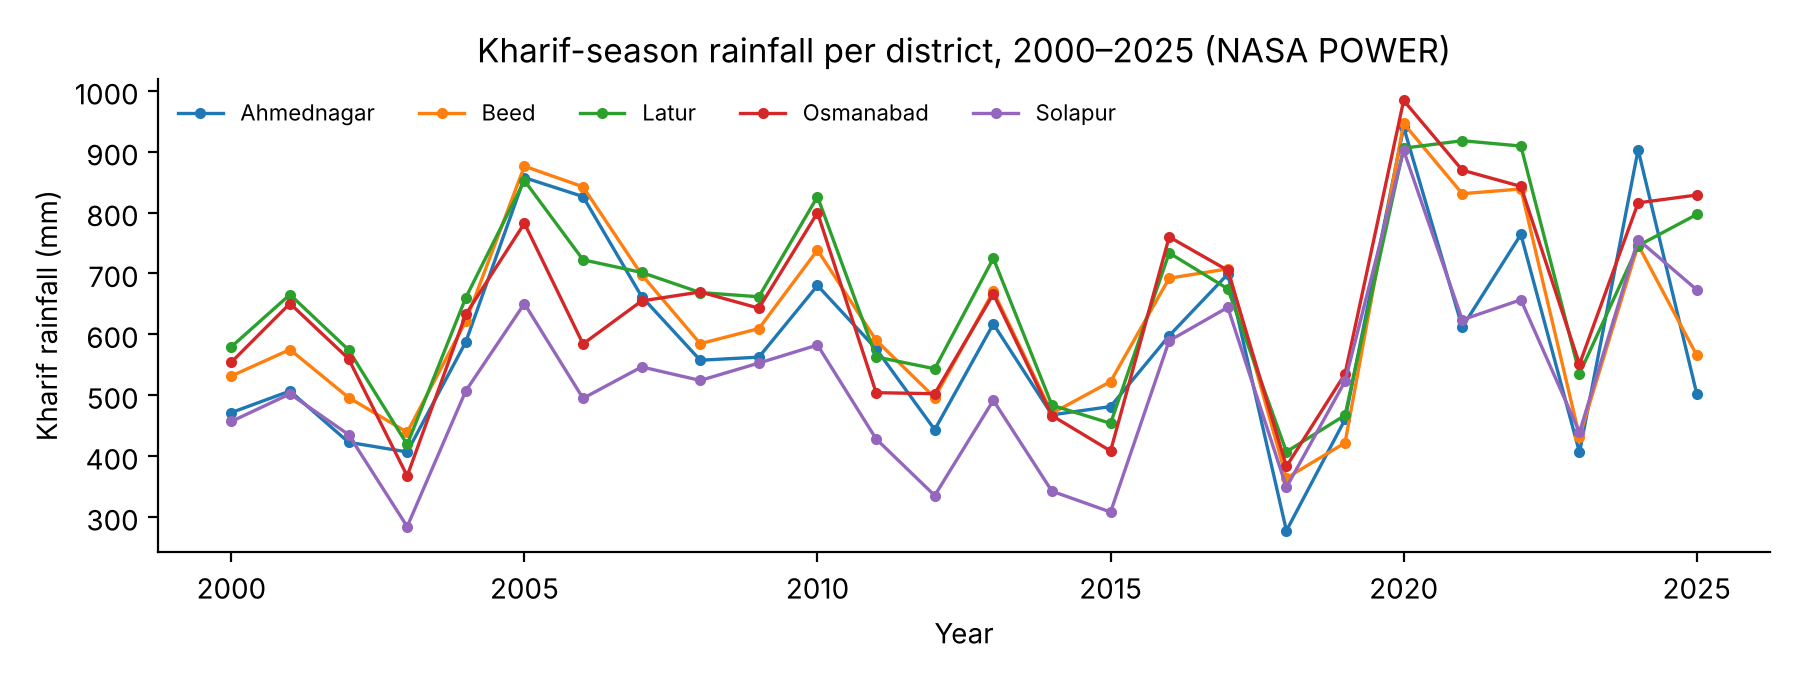
\includegraphics[width=\textwidth]{kharif_rain.png}
	\caption{Kharif-season rainfall in each district, 2000--2025. Dips such as 2014 and 2018 correspond to known drought years.}
	\label{fig:kharifrain}
\end{figure}

The exploratory analysis brought out several facts that shaped the design:
\begin{itemize}
	\item \textbf{High year-to-year variability.} Annual rainfall varies by 150 to 185 mm (about 20 to 25\%) around each district's mean. A drought must therefore be judged against the district's own history, not a fixed threshold.
	\item \textbf{Strong monsoon dependence.} Between 74 and 81\% of the annual rainfall falls in June to September. The other eight months are structurally dry, which supports aggregating weather to the season level for the yield model.
	\item \textbf{Extreme dry spells.} The longest recorded dry spell reaches 125 to 133 days in Solapur and Beed, more than four months without meaningful rain.
	\item \textbf{Rainfall is trending upward.} Comparing the first and the latest decade, annual rainfall rose by 2\% (Latur) to 16\% (Solapur), so models trained on older years may under-predict recent rainfall.
	\item \textbf{Temperature is fairly uniform} across districts: daily means of 25.7 to 26.8\,\textdegree C, summer highs near 44 to 45\,\textdegree C and winter lows of 7 to 9\,\textdegree C.
\end{itemize}

\section{Data sources}
The project uses four public data sources, summarised in Table~\ref{tab:sources}.

\begin{table}[H]
	\centering
	\caption{Data sources used in the project}
	\label{tab:sources}
	\small
	\begin{tabularx}{\textwidth}{p{3.2cm}p{3.3cm}YY}
		\toprule
		\textbf{Source} & \textbf{Coverage} & \textbf{Content} & \textbf{Used for} \\
		\midrule
		NASA POWER \cite{nasapower} daily weather & 1 Jan 2000 -- 31 Dec 2025, one file per district & 11 daily variables: rainfall, mean/max/min temperature, relative humidity, wind speed at 2\,m and 50\,m, surface pressure, solar radiation, dew point, cloud cover & Weather forecasting, season summaries, condition labelling \\
		DES district crop statistics \cite{desagri} & 2000--01 to 2022--23 & Area, production and yield per district, crop and season & Yield-model target; which crops each district grows \\
		ICAR-CRIDA District Agriculture Contingency Plans \cite{crida2011plans} & 5 PDFs, 2011 & District profile (rainfall normal, soils, land use, irrigation) and condition$\to$action tables & Knowledge graph \\
		Census of India 2011 \cite{census2011} & District level & Population, density, sex ratio, decadal growth; total workers 1991/2001/2011 & Human-impact layer only \\
		\bottomrule
	\end{tabularx}
\end{table}

\subsection{Weather data}
The weather files come from NASA's POWER project, which provides daily values derived from satellite observations and reanalysis on a regular grid. Each district file has one row per day from 2000 to 2025 (about 9,500 rows) and, after cleaning, no missing dates. Because POWER values are grid averages, they smooth out local extremes: a cloudburst over one village is spread over the whole cell. This matters later when heavy-rain events are labelled (Chapter~\ref{chap.6}).

\subsection{Crop statistics}
District-wise area, production and yield come from the Directorate of Economics and Statistics (DES), Ministry of Agriculture and Farmers Welfare. Table~\ref{tab:crops} summarises the crop-season combinations available.

\begin{table}[H]
	\centering
	\caption{Crop-season combinations in the DES data (five districts, 2000--01 to 2022--23)}
	\label{tab:crops}
	\begin{tabular}{lccc}
		\toprule
		\textbf{Crop (season)} & \textbf{Mean area (ha)} & \textbf{Mean yield (t/ha)} & \textbf{Missing} \\
		\midrule
		Arhar/Tur (Kharif) & 54,261 & 0.61 & 0\% \\
		Bajra (Kharif) & 71,562 & 0.53 & 0.9\% \\
		Jowar (Kharif) & 40,904 & 0.78 & 7.0\% \\
		Jowar (Rabi) & 305,949 & 0.64 & 0\% \\
		Soybean (Kharif) & 109,932 & 1.07 & 0\% \\
		Sunflower (Kharif) & 8,336 & 0.46 & 0.9\% \\
		Sunflower (Rabi) & 14,320 & 0.55 & 6.1\% \\
		\bottomrule
	\end{tabular}
\end{table}

Rabi Jowar is by far the largest crop by area (about 306,000 ha on average), and Soybean has the highest mean yield. Yields differ sharply between districts: Kharif Jowar averages 1.10 t/ha in Latur but only 0.56 t/ha in Solapur. Each district-crop-season has at most 23 yearly records, which is why deep learning is not used for yield.

\subsection{Contingency plans}
The five plans were prepared in 2010--2011 in a common ICAR template. Pages 1--2 contain the district profile: rainfall normal, soil types with their area, land use and irrigated area. Section 2, "Strategies for weather related contingencies", contains the condition$\to$action tables that form the heart of the knowledge graph (Chapter~\ref{chap.6}). Table~\ref{tab:profile} shows the profile values extracted from them.

\begin{table}[H]
	\centering
	\caption{District profile extracted from the contingency plans}
	\label{tab:profile}
	\small
	\setlength{\tabcolsep}{4pt}\begin{tabular}{lccl}
		\toprule
		\textbf{District} & \textbf{Rainfall normal (mm)} & \textbf{Net irrigated area} & \textbf{Dominant soil (share of area)} \\
		\midrule
		Ahmednagar & 419.0 & not stated & Shallow grey soils (389 kha) \\
		Beed       & 605.4 & 16.0\% & Shallow black soils (58.9\%) \\
		Latur      & 634.9 & not captured & Shallow soils (49.4\%) \\
		Osmanabad  & 693.9 & 15.6\% & Shallow soils (66.1\%) \\
		Solapur    & 550.5 & not stated & Shallow black soil (67.8\%) \\
		\bottomrule
	\end{tabular}
\end{table}

\subsection{Census data}
Census 2011 tables give each district's population, density, sex ratio and decadal growth, and the total number of workers in 1991, 2001 and 2011. These are used only \emph{after} a yield has been predicted, to estimate how many people are exposed to a loss. They are never used as yield-model features, because there is no agronomic reason why population should change yield, and adding such features to a model trained on about 23 points per crop would invite spurious fits.

\section{Data audit and preprocessing}
Before any modelling, every file was opened and checked. The main problems found, and how they were handled, are listed below.

\begin{enumerate}
	\item \textbf{Mislabelled files.} The DES and Census ".xls" files are actually HTML pages saved with an Excel extension. They are read with \texttt{pandas.read\_html} and saved as clean CSV files.
	\item \textbf{Inconsistent district names.} The same district is spelt differently in different sources (Table~\ref{tab:names}). A single mapping module (\texttt{district\_name\_map.py}) translates every spelling to one canonical name.
	\item \textbf{Inconsistent crop names.} DES says "Bajra" while the plans say "Pearl millet" or "Pearlmillet"; "Tur", "Arhar" and "Pigeon pea" are the same crop. The same module maps crop names and their aliases.
	\item \textbf{Agricultural years.} DES reports years as "2000--2001". These are converted to an integer crop year for joining with weather.
	\item \textbf{Genuine gaps.} Some DES cells are empty (for example Ahmednagar Kharif Jowar from 2009--10 to 2015--16). These are reporting gaps, not zero yields, and are kept as missing.
	\item \textbf{Missing crop.} Rabi Gram (chickpea), an important crop in all five districts, is absent from the downloaded DES table and must be sourced separately.
	\item \textbf{Weather gaps.} The few gaps in the weather files are filled in the preprocessing notebook, which writes a clean copy used by all models. Rainfall and wind speed, which are highly skewed, are log-transformed before training.
	\item \textbf{Unrelated material.} One review document found in the shared folder belonged to a different project scope and was excluded.
\end{enumerate}

\begin{table}[H]
	\centering
	\caption{District name variants across sources}
	\label{tab:names}
	\begin{tabular}{llll}
		\toprule
		\textbf{Canonical} & \textbf{DES} & \textbf{Census 2011} & \textbf{Weather / plans} \\
		\midrule
		Ahmednagar & Ahilyanagar & Ahmadnagar & Ahmednagar \\
		Beed & Beed & Bid & Beed \\
		Osmanabad & Dharashiv & Osmanabad & Osmanabad \\
		Latur & Latur & Latur & Latur \\
		Solapur & Solapur & Solapur & Solapur \\
		\bottomrule
	\end{tabular}
\end{table}

\section{Summary}
The four sources together give 26 years of daily weather, 23 years of crop yields, the official expert guidance and the population base for every district. Their main weaknesses are known and recorded: daily rainfall is very skewed and hard to forecast, the crop records are short, Rabi Gram is missing, and the contingency plans and Census figures are single snapshots from 2011.

\chapter{System Architecture and Methodology}
\label{chap.4}
\section{Overview}
The system is a pipeline of ten stages grouped into four phases (Figure~\ref{fig:arch}). A user chooses a district and a season. The weather for the coming days is forecast, the season is summarised and classified, crop yield is predicted and explained, the loss is turned into human impact, and finally the matching official guidance is retrieved and explained in plain language. Each stage writes a well-defined output that the next stage reads, so stages can be built, tested and replaced independently.

\begin{figure}[H]
\centering
\resizebox{\textwidth}{!}{%
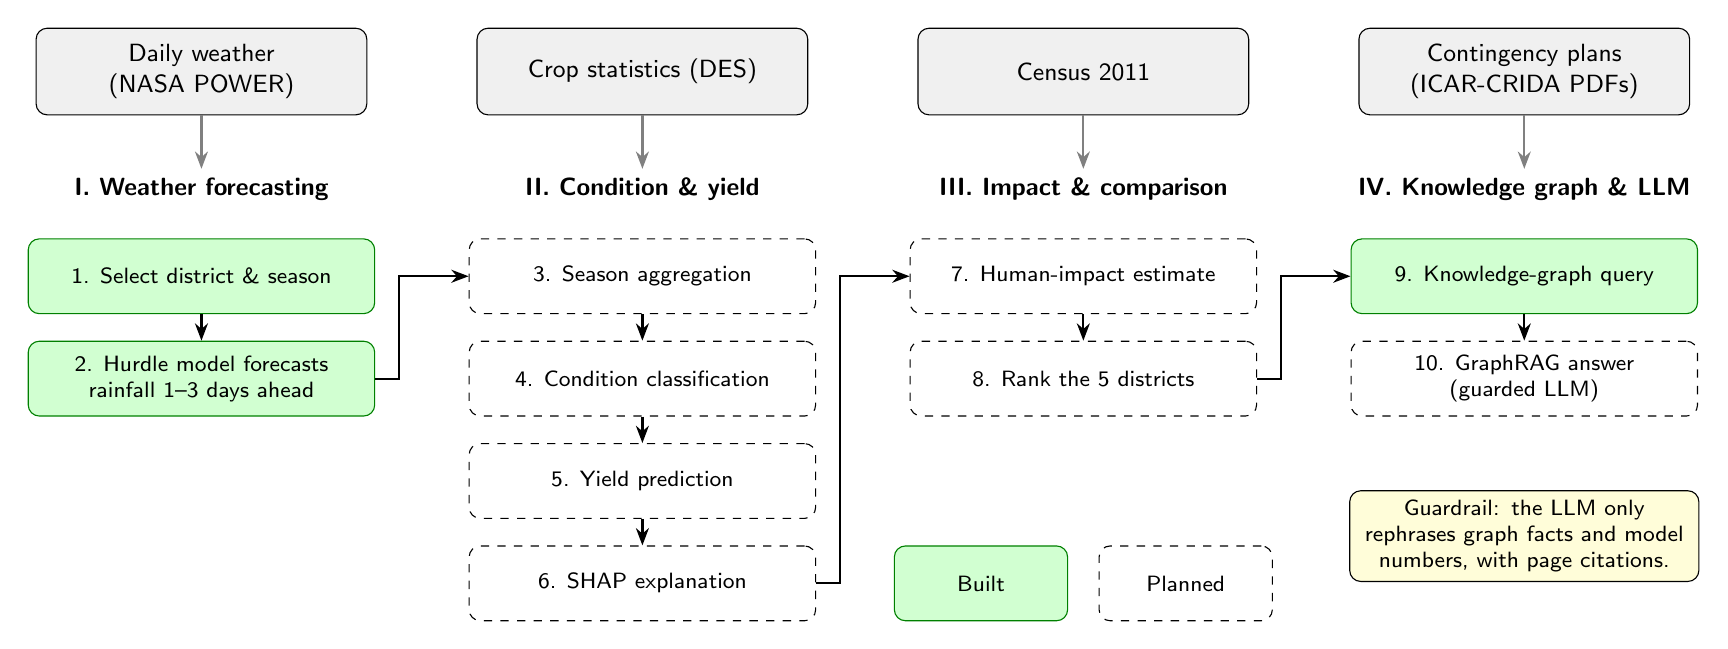
\begin{tikzpicture}[
  font=\sffamily\small,
  src/.style={draw, rounded corners, fill=gray!12, minimum width=4.2cm, minimum height=1.1cm, align=center},
  stg/.style={draw, rounded corners, minimum width=4.4cm, minimum height=0.95cm, align=center, font=\sffamily\footnotesize},
  done/.style={stg, fill=green!18, draw=green!50!black},
  plan/.style={stg, fill=white, dashed},
  ph/.style={font=\sffamily\bfseries\small, align=center},
  arr/.style={-{Stealth[length=2.2mm]}, thick}
]
\def\xa{0}\def\xb{5.6}\def\xc{11.2}\def\xd{16.8}
\node[src] (w) at (\xa,0) {Daily weather\\(NASA POWER)};
\node[src] (c) at (\xb,0) {Crop statistics (DES)};
\node[src] (k) at (\xc,0) {Census 2011};
\node[src] (p) at (\xd,0) {Contingency plans\\(ICAR-CRIDA PDFs)};
\node[ph] (h1) at (\xa,-1.5) {I. Weather forecasting};
\node[ph] (h2) at (\xb,-1.5) {II. Condition \& yield};
\node[ph] (h3) at (\xc,-1.5) {III. Impact \& comparison};
\node[ph] (h4) at (\xd,-1.5) {IV. Knowledge graph \& LLM};
\draw[arr, gray] (w) -- (h1); \draw[arr, gray] (c) -- (h2);
\draw[arr, gray] (k) -- (h3); \draw[arr, gray] (p) -- (h4);
\node[done] (s1) at (\xa,-2.6) {1. Select district \& season};
\node[done] (s2) at (\xa,-3.9) {2. Hurdle model forecasts\\rainfall 1--3 days ahead};
\node[plan] (s3) at (\xb,-2.6) {3. Season aggregation};
\node[plan] (s4) at (\xb,-3.9) {4. Condition classification};
\node[plan] (s5) at (\xb,-5.2) {5. Yield prediction};
\node[plan] (s6) at (\xb,-6.5) {6. SHAP explanation};
\node[plan] (s7) at (\xc,-2.6) {7. Human-impact estimate};
\node[plan] (s8) at (\xc,-3.9) {8. Rank the 5 districts};
\node[done] (s9) at (\xd,-2.6) {9. Knowledge-graph query};
\node[plan] (s10) at (\xd,-3.9) {10. GraphRAG answer\\(guarded LLM)};
\draw[arr] (s1) -- (s2);
\draw[arr] (s2.east) -- ++(0.3,0) |- (s3.west);
\draw[arr] (s3) -- (s4); \draw[arr] (s4) -- (s5); \draw[arr] (s5) -- (s6);
\draw[arr] (s6.east) -- ++(0.3,0) |- (s7.west);
\draw[arr] (s7) -- (s8);
\draw[arr] (s8.east) -- ++(0.3,0) |- (s9.west);
\draw[arr] (s9) -- (s10);
\node[draw, rounded corners, fill=yellow!15, align=center, font=\sffamily\footnotesize, text width=4.2cm] at (\xd,-5.9) {Guardrail: the LLM only rephrases graph facts and model numbers, with page citations.};
\node[done, minimum width=2.2cm] at (\xc-1.3,-6.5) {Built};
\node[plan, minimum width=2.2cm] at (\xc+1.3,-6.5) {Planned};
\end{tikzpicture}}
\caption{System architecture: ten stages in four phases. Green boxes are built; dashed boxes are planned for the second phase.}
\label{fig:arch}
\end{figure}

\section{The ten stages}
Table~\ref{tab:stages} describes what each stage does in plain terms and its status at the end of the first phase.

\begin{table}[H]
	\centering
	\caption{Pipeline stages and their status}
	\label{tab:stages}
	\small
	\begin{tabularx}{\textwidth}{clYl}
		\toprule
		\textbf{\#} & \textbf{Stage} & \textbf{What it does} & \textbf{Status} \\
		\midrule
		1 & Selection & The user chooses a district and a crop-season (Kharif or Rabi). & Done \\
		2 & Weather forecast & A two-stage hurdle model trained on that district's history forecasts daily rainfall 1 to 3 days ahead (LSTM, SARIMA, XGBoost and TFT were evaluated as comparative models). & Done \\
		3 & Season aggregation & Daily weather is summarised into season rainfall, longest dry spell, monsoon onset date, etc. & Planned \\
		4 & Condition classification & The season is labelled normal, dry spell, deficit or drought-like against the district's own history (SPI/terciles and the plans' definitions). & Planned$^\dagger$ \\
		5 & Yield prediction & Random forest / gradient boosting (with a linear baseline) predict yield per district, crop and season. & Planned \\
		6 & Explanation & SHAP shows which weather factors pushed each predicted yield up or down. & Planned \\
		7 & Human impact & The yield shortfall is converted into people and workers affected using Census data. & Planned \\
		8 & District comparison & Severity and exposure scores are normalised and combined to rank the five districts. & Planned \\
		9 & Knowledge-graph query & The graph returns the official actions for the district, crop, season and condition, with page citations. & Done \\
		10 & GraphRAG answer & An LLM extracts entities from a question, retrieves the subgraph and writes one grounded answer. & Planned \\
		\bottomrule
	\end{tabularx}
	\\[2pt]
	\footnotesize $^\dagger$ A rule-based season labeller built for the knowledge graph already labels all past seasons and acts as a stand-in for Stage~4 (Section~\ref{sec:labeller}).
\end{table}

\section{Key design decisions}
\begin{enumerate}
	\item \textbf{One model per district.} The five districts have different rainfall regimes (Table~\ref{tab:climate}). Training a separate forecaster for each lets every model learn its own district's seasonality and avoids one district's patterns dominating another's.
	\item \textbf{Self-trained forecasting.} The forecast is produced from the district's own historical record, so the system keeps working without depending on an external live weather service.
	\item \textbf{A model built for rainfall.} Daily rainfall is zero on most days and highly skewed when it rains, so the main forecaster is a two-stage hurdle model that predicts rain occurrence and amount separately. Deep learning (LSTM, TFT) was evaluated in a comparative study; for the yield stage, with only about 23 seasons per district-crop, tree ensembles and a linear baseline are used.
	\item \textbf{History-relative drought.} Conditions are judged against each district's own 2000--2025 record and the plans' own definitions, never against one national threshold.
	\item \textbf{Census only after prediction.} Population and workforce enter only the impact stage, never the yield model.
	\item \textbf{Structured knowledge, not free text.} The contingency plans are turned into a graph whose every edge records the source page, so any recommendation can be traced.
	\item \textbf{A guarded LLM.} The LLM sees only retrieved graph facts and model outputs, and its job is to phrase them clearly.
	\item \textbf{Replaceable stages with fixed interfaces.} For example, the graph reads season labels from a CSV with fixed columns; when Stage~4 is built it simply writes a file with the same columns, and the graph picks it up with no change to its schema.
\end{enumerate}

\section{How a query flows through the system}
The following example shows how the finished system is intended to answer a question; Stages 2 and 9 already work today.

\begin{enumerate}
	\item \textbf{Question:} "Rain has stopped in Beed for two weeks while the soybean is flowering. What should be done?"
	\item \textbf{Stage 10} extracts the entities: district = Beed, crop = Soybean, season = Kharif, condition = mid-season dry spell at flowering.
	\item \textbf{Stages 2--4} confirm the condition from the forecast and the season-to-date weather.
	\item \textbf{Stages 5--8} predict the soybean yield for the season, explain the drivers, estimate the people affected and place Beed in the district ranking.
	\item \textbf{Stage 9} retrieves the Beed plan's recommendations for this situation, for example "give protective irrigation with sprinkler" (Beed plan, p.~18), together with past seasons in which Beed had the same condition and the yield that followed.
	\item \textbf{Stage 10} writes one answer from these pieces only, citing the plan pages.
\end{enumerate}

\section{Technology stack}
\begin{itemize}
	\item \textbf{Language and data:} Python, pandas, NumPy; Jupyter notebooks for exploration.
	\item \textbf{Forecasting:} scikit-learn \cite{pedregosa2011scikit} for the main hurdle model; for the comparative study, PyTorch \cite{paszke2019pytorch} (LSTM, TFT), XGBoost and statsmodels (SARIMA).
	\item \textbf{Knowledge graph:} pdfplumber for table extraction, NetworkX \cite{hagberg2008exploring} for the graph, GraphML/JSON export, Neo4j import scripts, vis-network for the interactive viewer.
	\item \textbf{MLOps:} Git and GitHub Actions, DVC with a DagsHub remote, MLflow \cite{zaharia2018accelerating} model registry, FastAPI service, Docker, pytest.
	\item \textbf{Planned:} SHAP for explanations; LangChain/LlamaIndex for GraphRAG; Streamlit for the user interface.
\end{itemize}

\chapter{Weather Forecasting}
\label{chap.5}
\section{What this stage has to do}
Stage 2 takes the recent daily weather of a district and forecasts the coming days. Its output feeds the season summary (Stage 3): to judge whether the current season is heading into a dry spell or a delayed onset, the system needs both the weather observed so far and a view of the days ahead. The forecasting model has to work without calling an external weather service, so it is trained only on the district's own 26-year record.

Of all the weather variables, \textbf{rainfall} matters most here. Every condition in the contingency plans (delayed onset, dry spell, terminal drought, excess rain) is defined by rainfall, and rainfall is the main weather driver of rainfed crop yield. The project therefore uses a model designed specifically for daily rainfall, the \textbf{two-stage hurdle model}, as its \textbf{main forecasting model}, used one per district throughout the pipeline. Four other well-known approaches, an LSTM network, SARIMA, XGBoost and a Temporal Fusion Transformer, were trained on the same data as a \textbf{comparative study}, to check that the choice of the hurdle model is justified.

One rule applies to every model in this chapter: a forecast may use only information that would really be available on the day the forecast is made.

\section{Why daily rainfall needs a special model}
Daily rainfall behaves very differently from smooth variables such as temperature (Figure~\ref{fig:raindist}):
\begin{itemize}
	\item \textbf{Most days are dry.} In every district about 62--64\% of days have no measurable rain (0.25\,mm or less), and 80--83\% have less than 2.5\,mm, the India Meteorological Department's threshold for a "rainy day".
	\item \textbf{The rain that does fall is highly skewed.} On rainy days the median amount is only about 2--3\,mm, yet the heaviest 10\% of rainy days deliver about 42--44\% of all the rain.
\end{itemize}
A model that predicts rainfall as one continuous number, and is trained to keep its average error small, learns a poor compromise: it predicts "a little rain" on almost every day. That is never badly wrong on dry days, but it blurs the difference between dry and wet days and badly under-predicts heavy rain. Both are exactly what a drought system needs to get right.

\begin{figure}[H]
	\centering
	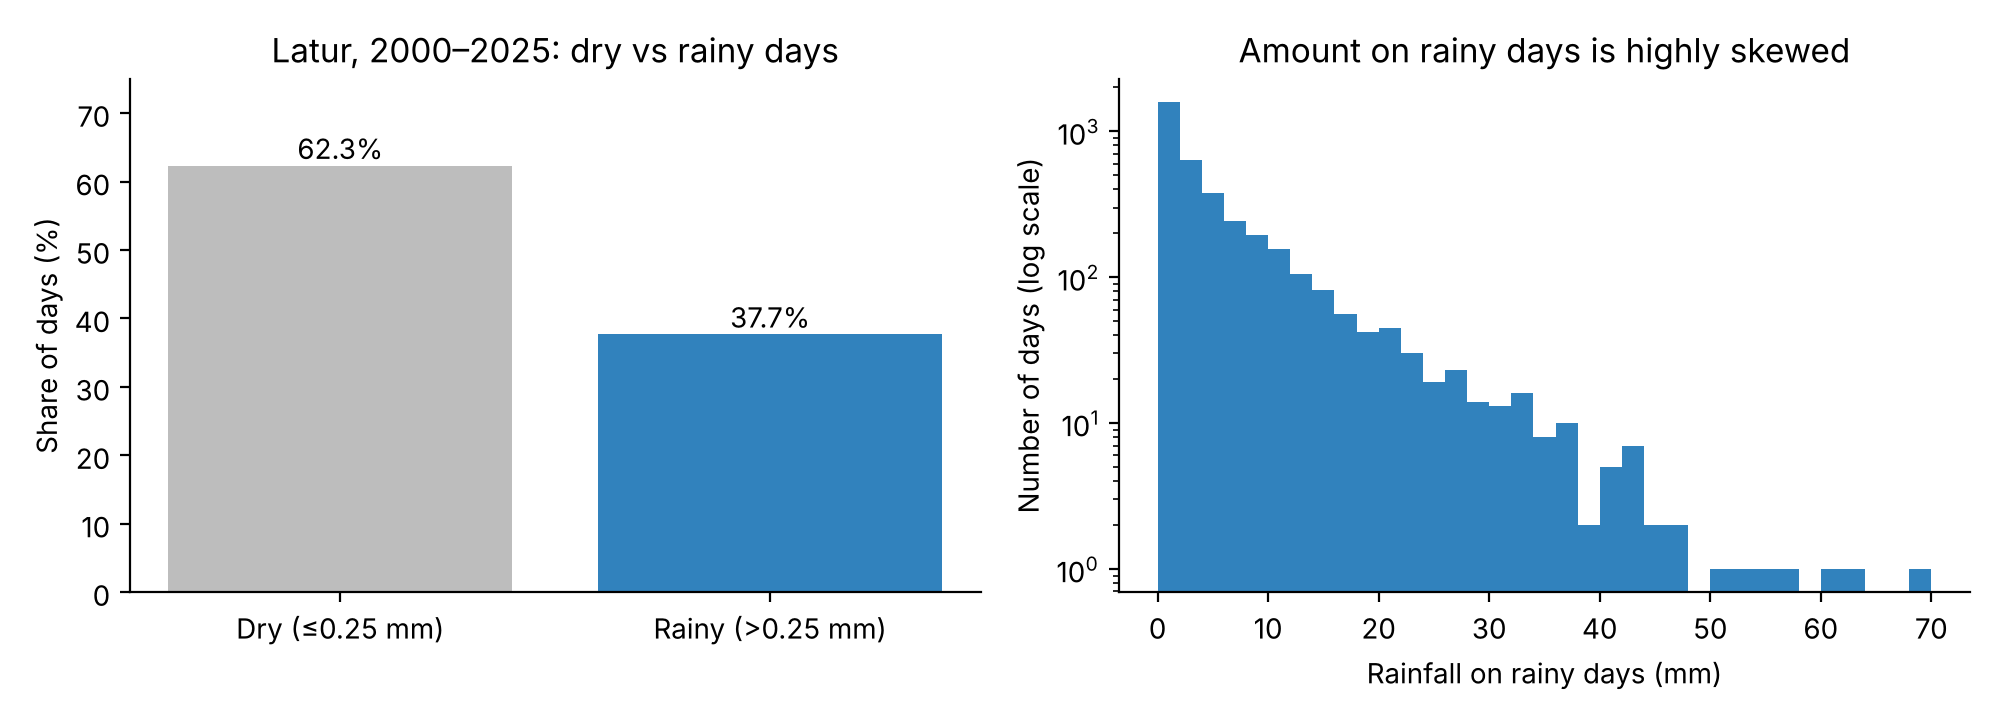
\includegraphics[width=\textwidth]{rain_distribution.png}
	\caption{Daily rainfall in Latur, 2000--2025. Left: about 62\% of days are dry. Right: rainy-day amounts are heavily skewed (note the log scale). The other four districts look the same.}
	\label{fig:raindist}
\end{figure}

Statisticians have long modelled such variables in two parts: first \emph{whether} the event happens, then \emph{how large} it is given that it happens \cite{cragg1971some,mullahy1986specification}. Classical daily-rainfall models do the same, pairing a wet/dry occurrence process with a separate distribution for the amount \cite{stern1984model}. The hurdle model follows this idea.

\section{Evaluation set-up}

\subsection{Chronological split}
Weather is a time series, so data are never shuffled; every model is trained on the past and tested on a later period it has never seen. For the hurdle model the split is made on the date being forecast (the \emph{target} date):
\begin{itemize}
	\item \textbf{Test:} target dates from 1 January 2022 onwards (about 1,718 days per horizon); all results below are on this period;
	\item \textbf{Validation:} the 365 days before the test period;
	\item \textbf{Training:} everything earlier, from 2000.
\end{itemize}

\subsection{Metrics}
For $n$ test days with observed values $y_t$, forecasts $\hat{y}_t$ and observed mean $\bar{y}$:
\begin{align}
	\text{RMSE} &= \sqrt{\frac{1}{n}\sum_{t=1}^{n}(y_t-\hat{y}_t)^2}, \qquad
	\text{MAE} = \frac{1}{n}\sum_{t=1}^{n}\lvert y_t-\hat{y}_t\rvert, \\
	R^2 &= 1-\frac{\sum_{t}(y_t-\hat{y}_t)^2}{\sum_{t}(y_t-\bar{y})^2}.
\end{align}
RMSE and MAE are in millimetres; RMSE punishes large misses more heavily. $R^2$ is unit-free: 1 means perfect, 0 means no better than always predicting the test-period average, and negative values mean worse than that. For daily rainfall a few heavy days dominate the sum of squares, so even a useful model has a modest $R^2$.

\section{The hurdle model (main model)}

\subsection{Structure}
For each district and each forecast horizon $h \in \{1,2,3\}$ days, the model has two parts (Figure~\ref{fig:hurdle}):
\begin{enumerate}
	\item \textbf{Hurdle 1, the rain gate.} A gradient-boosted classifier estimates the probability $p$ that day $t+h$ will have more than 0.25\,mm of rain.
	\item \textbf{Hurdle 2, the rain depth.} A gradient-boosted regressor, trained only on rainy days, predicts $\log(1+\text{rainfall})$ on day $t+h$. Working on the log scale tames the skew of heavy events.
\end{enumerate}
The forecast combines the two:
\begin{equation}
	\hat{y}_{t+h} =
	\begin{cases}
		\exp\big(g_h(\mathbf{x}_t)\big) - 1 & \text{if } p_h(\mathbf{x}_t) > \tau,\\
		0 & \text{otherwise,}
	\end{cases}
	\qquad \tau = 0.35,
\end{equation}
where $\mathbf{x}_t$ are the features available on forecast day $t$, $p_h$ is the gate and $g_h$ the depth model. The threshold $\tau = 0.35$ is set below 0.5 on purpose: because rainy days are the minority, a gate that waited for 50\% certainty would miss too many of them. Training separate models for each horizon (\emph{direct} multi-step forecasting) avoids feeding one day's forecast into the next, which would compound errors.

\begin{figure}[H]
\centering
\resizebox{\textwidth}{!}{%
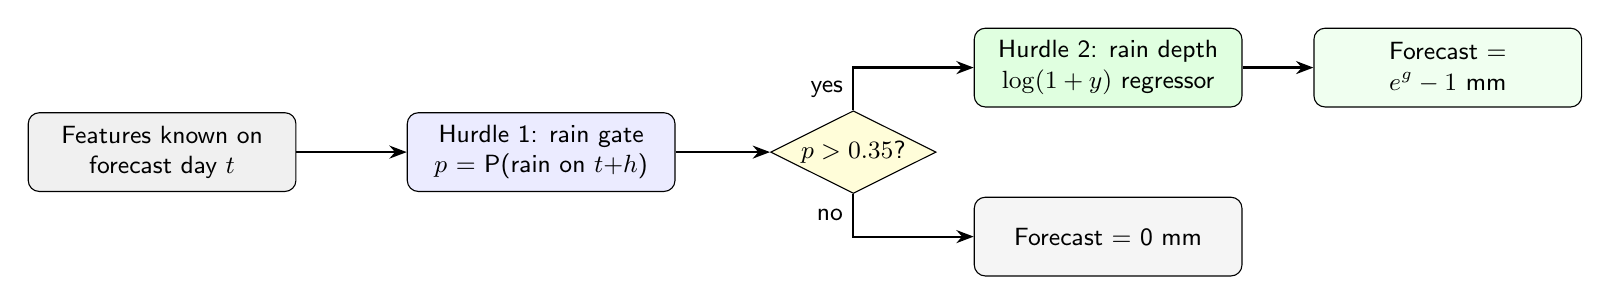
\begin{tikzpicture}[
  font=\sffamily\small,
  box/.style={draw, rounded corners, minimum width=3.4cm, minimum height=1.0cm, align=center},
  arr/.style={-{Stealth[length=2.2mm]}, thick}
]
\node[box, fill=gray!12] (x) {Features known on\\forecast day $t$};
\node[box, fill=blue!8, right=1.4cm of x] (g) {Hurdle 1: rain gate\\$p$ = P(rain on $t{+}h$)};
\node[draw, diamond, aspect=2, fill=yellow!15, right=1.2cm of g, align=center, inner sep=1pt] (d) {$p > 0.35$?};
\node[box, fill=green!12, above right=0.3cm and 1.0cm of d] (r) {Hurdle 2: rain depth\\$\log(1+y)$ regressor};
\node[box, fill=gray!8, below right=0.3cm and 1.0cm of d] (z) {Forecast = 0 mm};
\node[box, fill=green!6, right=0.9cm of r] (o) {Forecast =\\$e^{g}-1$ mm};
\draw[arr] (x) -- (g); \draw[arr] (g) -- (d);
\draw[arr] (d.north) |- node[pos=0.25, left]{yes} (r.west);
\draw[arr] (d.south) |- node[pos=0.25, left]{no} (z.west);
\draw[arr] (r) -- (o);
\end{tikzpicture}}
\caption{The two-stage hurdle model. One gate and one depth model are trained for each district and each horizon $h = 1, 2, 3$ days.}
\label{fig:hurdle}
\end{figure}

\subsection{Features}
Every feature is computed only from data available on the forecast day $t$; rolling rainfall statistics end on the day \emph{before} $t$, so they never include the rain being predicted. The 21 features are:
\begin{itemize}
	\item \textbf{Season:} $\sin(2\pi d/365.25)$ and $\cos(2\pi d/365.25)$ of the day of year $d$, which tell the model where it is in the monsoon cycle and place 31 December next to 1 January;
	\item \textbf{Recent rain:} rainfall 1, 2 and 3 days earlier; mean rainfall over the previous 3, 7 and 14 days; maximum rainfall in the previous 3 days;
	\item \textbf{Moisture and pressure tendency:} humidity and pressure on the previous day and their day-to-day change; a falling pressure and rising humidity often precede rain;
	\item \textbf{Current conditions:} relative humidity, surface pressure, mean, maximum and minimum temperature, wind speed, solar radiation and dew point.
\end{itemize}

\subsection{Training settings}
Both parts use scikit-learn's histogram-based gradient boosting \cite{pedregosa2011scikit}: the gate with 250 boosting iterations and a learning rate of 0.04, the depth model with 350 iterations and a learning rate of 0.03, both with L2 regularisation of 0.1 and a fixed random seed. All settings live in one configuration file (Appendix~\ref{app:config}). Training needs no GPU and runs quickly on an ordinary laptop CPU, which makes regular retraining practical (Chapter~\ref{chap.7}).

\subsection{Model development: from nowcast to forecast}
\label{sec:leak}
The first version of the hurdle model also used physically motivated features (temperature range, dew-point spread, wind shear, vapour pressure deficit and a moisture-flux proxy) and a rule that set rainfall to zero when the air was clearly too dry. It scored very highly, with $R^2$ between 0.79 and 0.94. A careful review while building the MLOps pipeline showed why: its rolling rainfall features included the day being predicted, its humidity and temperature inputs were from that same day, and its target was same-day rainfall. In other words, it estimated today's rain from today's weather, a \emph{nowcast}, and was partly told the answer. This is a classic case of \emph{data leakage} \cite{kaufman2012leakage}. Figure~\ref{fig:hurdlev1} shows the symptom: the predicted series traces the observed one almost perfectly and with no delay, which no genuine forecast of daily rain can do.

\begin{figure}[H]
	\centering
	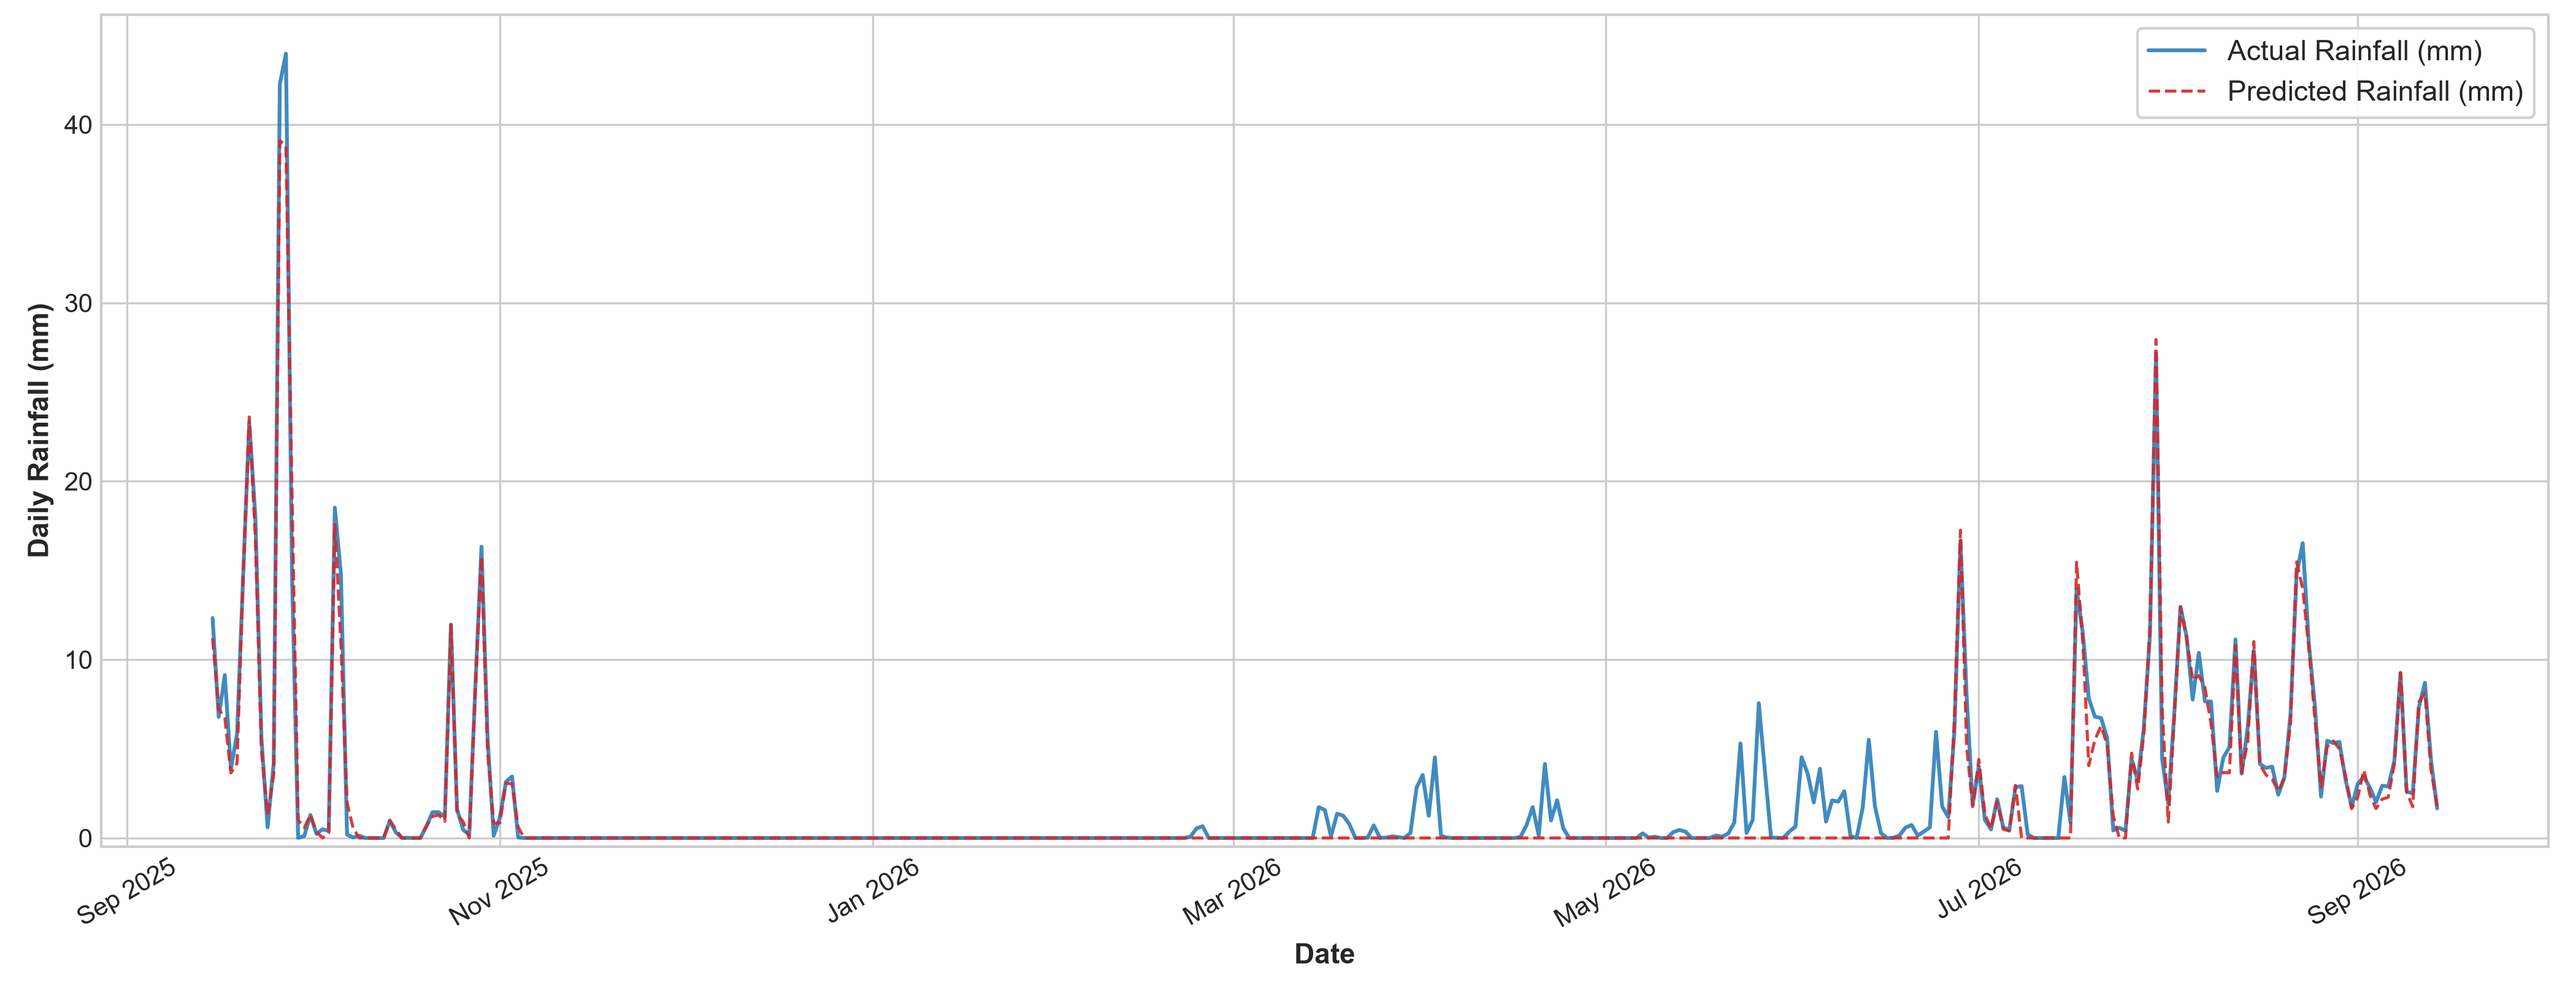
\includegraphics[width=\textwidth]{hurdle_v1_latur.png}
	\caption{First (same-day) version of the hurdle model, Latur, one-year validation window ($R^2 = 0.94$, RMSE 1.17\,mm, MAE 0.51\,mm). Because its inputs included the same day's rainfall, it reproduces the observed series almost exactly; it is a nowcast, not a forecast. The corresponding values for the other districts were $R^2$ 0.92 (Ahmednagar), 0.94 (Beed), 0.88 (Osmanabad) and 0.79 (Solapur).}
	\label{fig:hurdlev1}
\end{figure}

The model was therefore rebuilt as a genuine forecaster: features shifted so they end before the forecast day, targets moved $h$ days ahead, separate models per horizon, and the split made on the target date. All results in this chapter are for this corrected version, which is the one used in the project.

\subsection{Results}
Table~\ref{tab:hurdle} gives the test results for all five districts and all three horizons.

\begin{table}[H]
	\centering
	\caption{Hurdle model: rainfall forecast test results (target dates from 2022 onward)}
	\label{tab:hurdle}
	\small
	\begin{tabular}{lccccccccc}
		\toprule
		& \multicolumn{3}{c}{\textbf{Day +1}} & \multicolumn{3}{c}{\textbf{Day +2}} & \multicolumn{3}{c}{\textbf{Day +3}} \\
		\cmidrule(lr){2-4}\cmidrule(lr){5-7}\cmidrule(lr){8-10}
		\textbf{District} & $R^2$ & RMSE & MAE & $R^2$ & RMSE & MAE & $R^2$ & RMSE & MAE \\
		\midrule
		Ahmednagar & 0.151 & 7.09 & 1.62 & 0.103 & 7.29 & 1.74 & 0.072 & 7.41 & 1.80 \\
		Beed       & 0.259 & 4.74 & 1.62 & 0.190 & 4.96 & 1.77 & 0.147 & 5.08 & 1.77 \\
		Latur      & 0.289 & 4.50 & 1.80 & 0.186 & 4.81 & 1.99 & 0.154 & 4.91 & 2.04 \\
		Osmanabad  & 0.261 & 4.72 & 1.89 & 0.173 & 4.99 & 2.04 & 0.134 & 5.10 & 2.10 \\
		Solapur    & 0.282 & 4.12 & 1.59 & 0.150 & 4.49 & 1.73 & 0.106 & 4.60 & 1.82 \\
		\bottomrule
	\end{tabular}
	\\[2pt]
	\footnotesize RMSE and MAE in mm/day.
\end{table}

\begin{figure}[H]
	\centering
	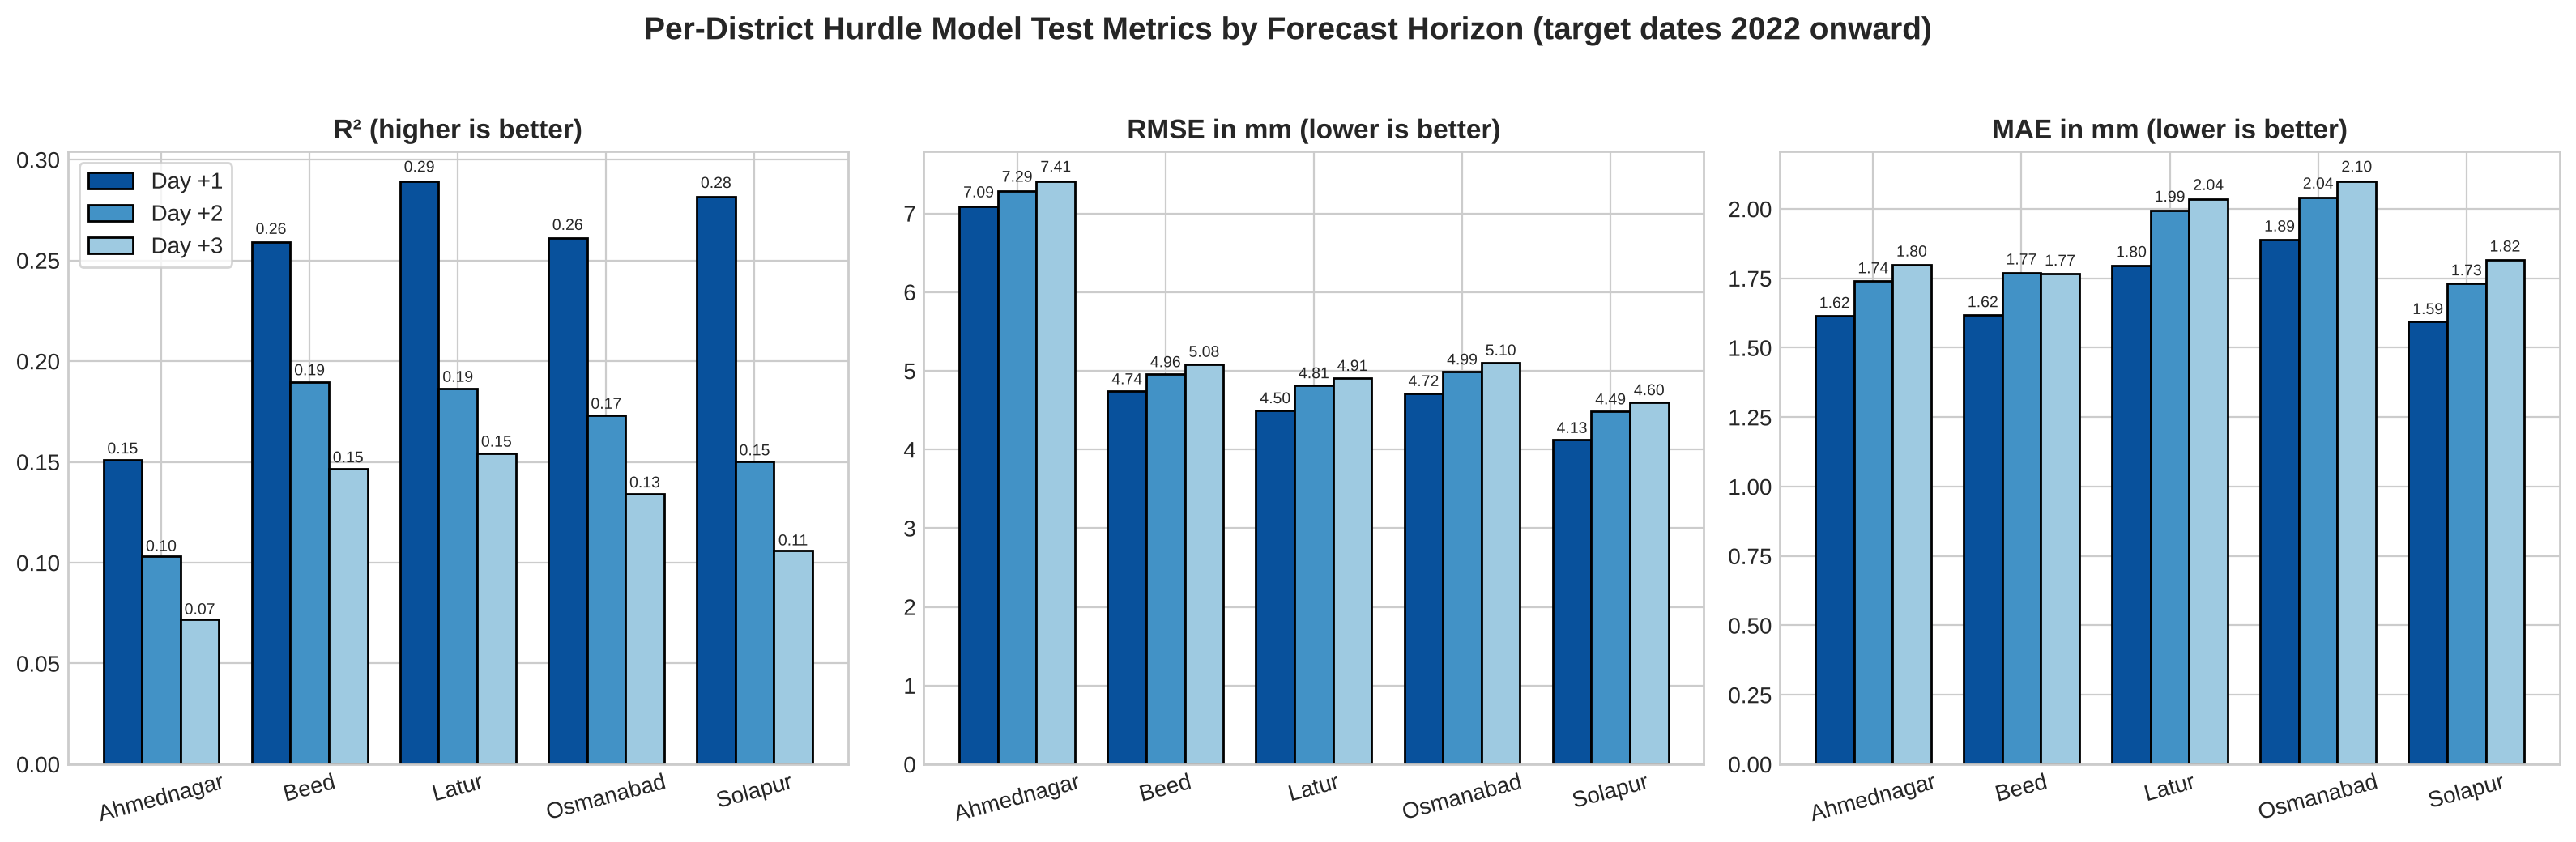
\includegraphics[width=\textwidth]{hurdle_metrics_summary.png}
	\caption{Hurdle model test metrics for each district and forecast horizon.}
	\label{fig:hurdlemetrics}
\end{figure}

\begin{itemize}
	\item \textbf{One day ahead}, the model explains 26--29\% of the day-to-day variation in rainfall in four of the five districts, with a typical error (MAE) of 1.6--1.9\,mm.
	\item \textbf{Skill falls with lead time}, to 0.07--0.15 by day 3. This is expected for point rainfall in a monsoon climate: whether it rains on a particular day a few days ahead is hard to predict from local history alone.
	\item \textbf{Ahmednagar is the hardest district.} Its RMSE is much larger because its record contains a few extreme events (one day exceeds 250\,mm) that dominate the squared error.
\end{itemize}

\paragraph{How well the gate separates dry and rainy days.} Because the drought rules in the plans depend on runs of dry days, the most important job of the model is to say correctly whether a day will be dry or rainy. Figure~\ref{fig:gate} evaluates Hurdle~1 on its own. One day ahead it classifies 84--88\% of days correctly and detects 89--92\% of rainy days; by day 3 accuracy is still 81--86\% and 84--87\% of rainy days are caught. About one in five of its "rain" calls turns out dry (18--26\% false alarms), which is the price of the deliberately low threshold $\tau = 0.35$: the gate prefers to catch rainy days, because a missed rainy day would wrongly extend a dry-spell count.

\begin{figure}[H]
	\centering
	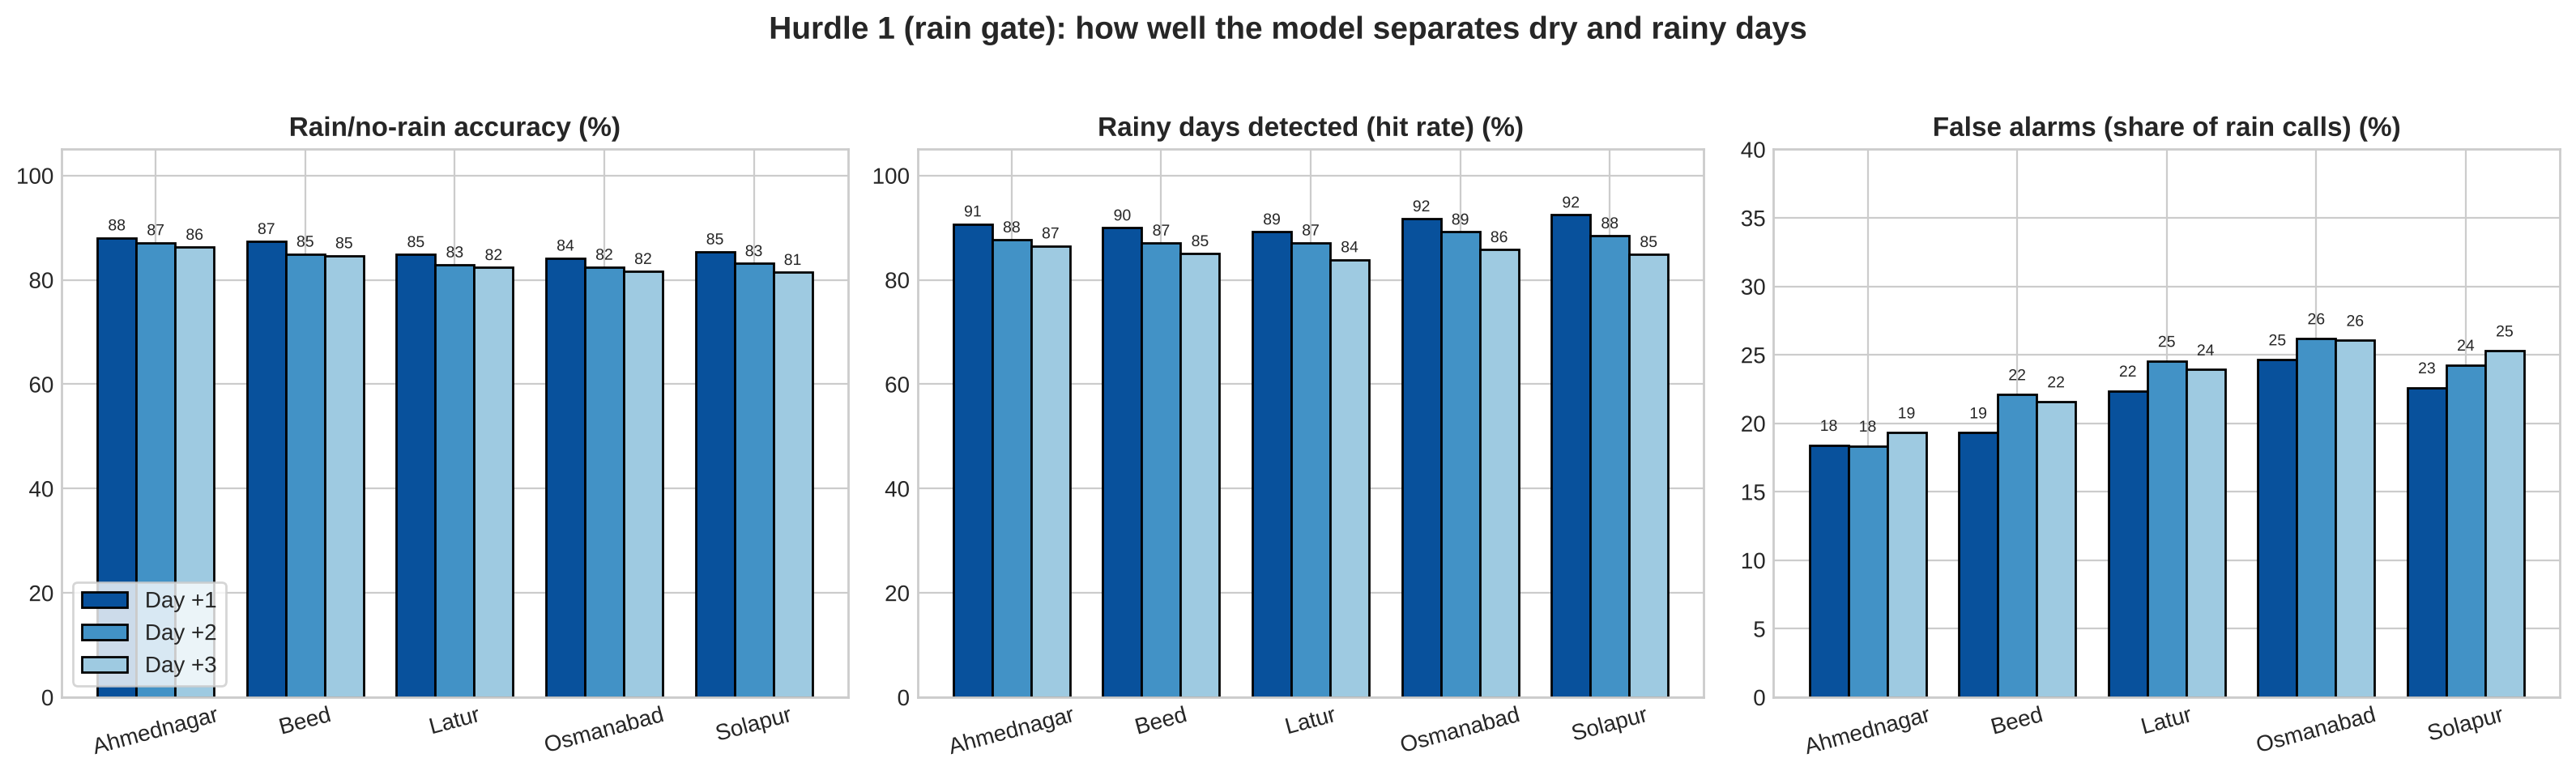
\includegraphics[width=\textwidth]{hurdle_gate_performance.png}
	\caption{Rain gate (Hurdle 1) on the test period: overall accuracy, share of rainy days detected, and share of rain forecasts that turned out dry.}
	\label{fig:gate}
\end{figure}

\paragraph{Forecasts over time.} Figure~\ref{fig:hurdleall} shows the one-day-ahead forecasts for all five districts over the last twelve months of the test period, and Figure~\ref{fig:hurdlelatur} zooms into the 2025 Kharif season in Latur. The model correctly keeps forecasts at zero through the dry months, and during the monsoon it follows wet and dry spells, but it rounds off the peaks: a 40\,mm day is typically forecast as 5--15\,mm, and the three-day-ahead forecast is smoother still.

\begin{figure}[H]
	\centering
	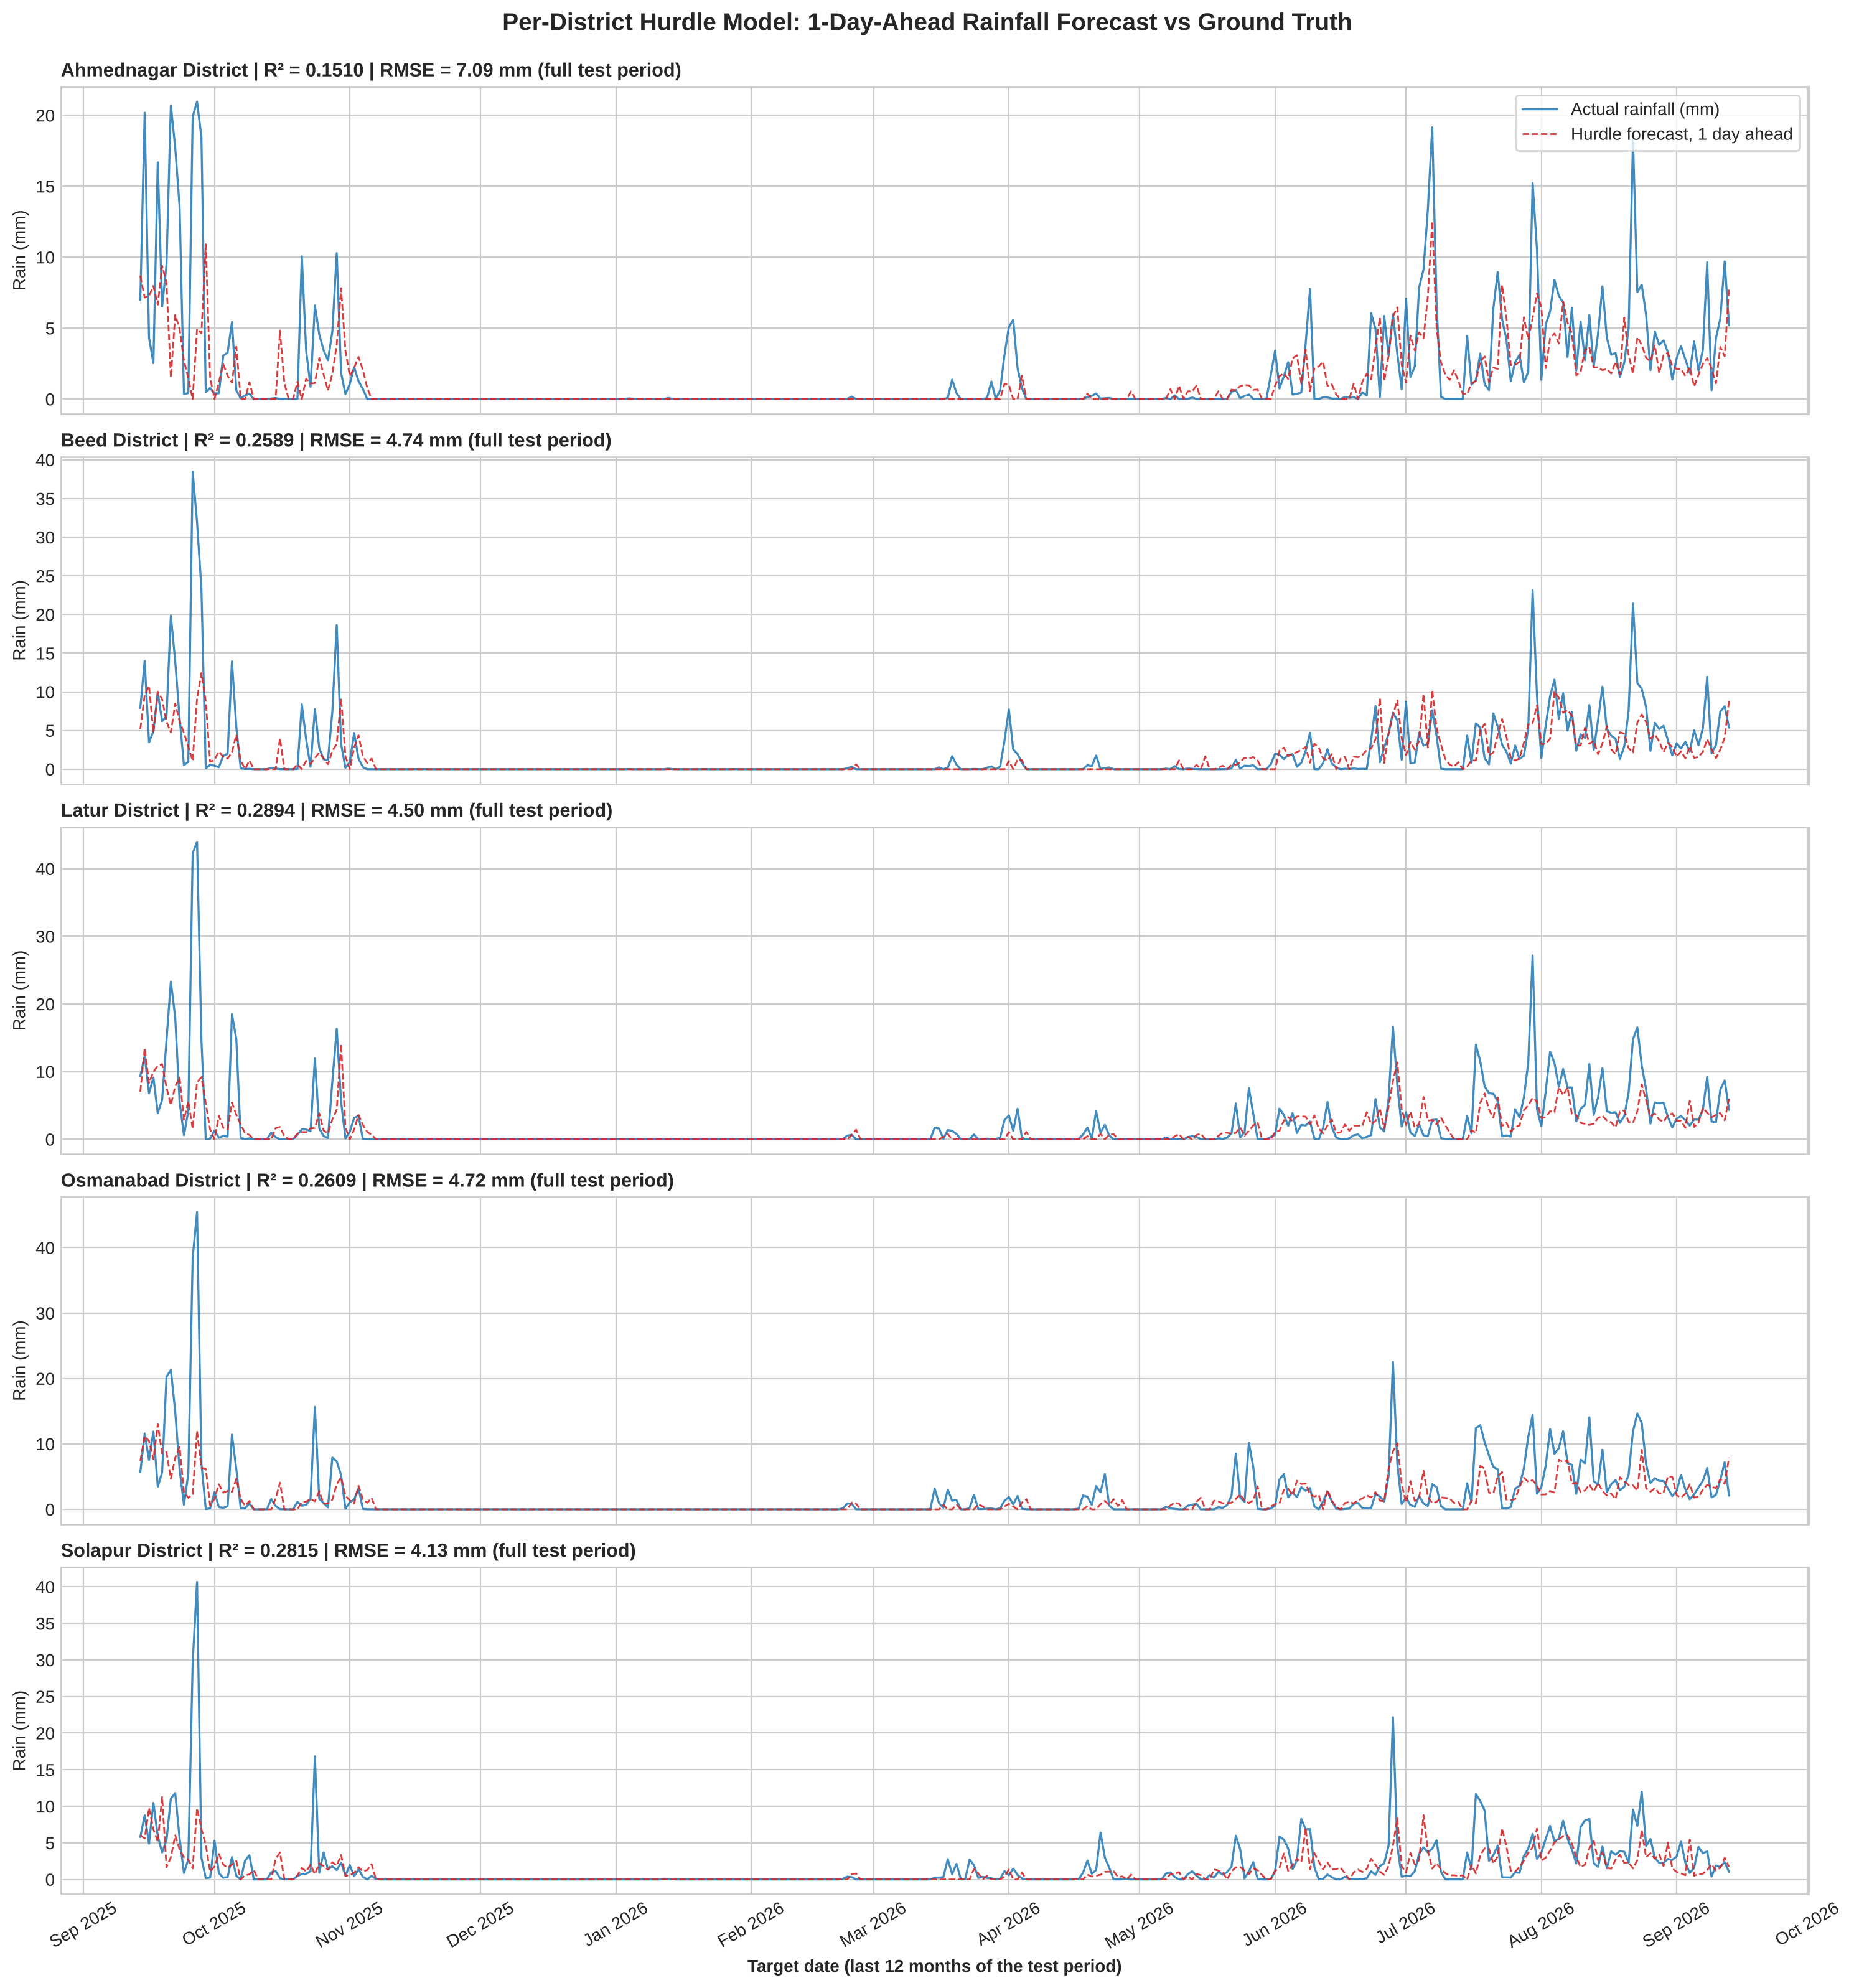
\includegraphics[width=0.97\textwidth,height=0.8\textheight,keepaspectratio]{hurdle_forecast_all_districts.png}
	\caption{Hurdle model: one-day-ahead rainfall forecast against observed rainfall for each district, September 2025 to September 2026. $R^2$ and RMSE in the panel titles are for the full test period (2022 onward).}
	\label{fig:hurdleall}
\end{figure}

\begin{figure}[H]
	\centering
	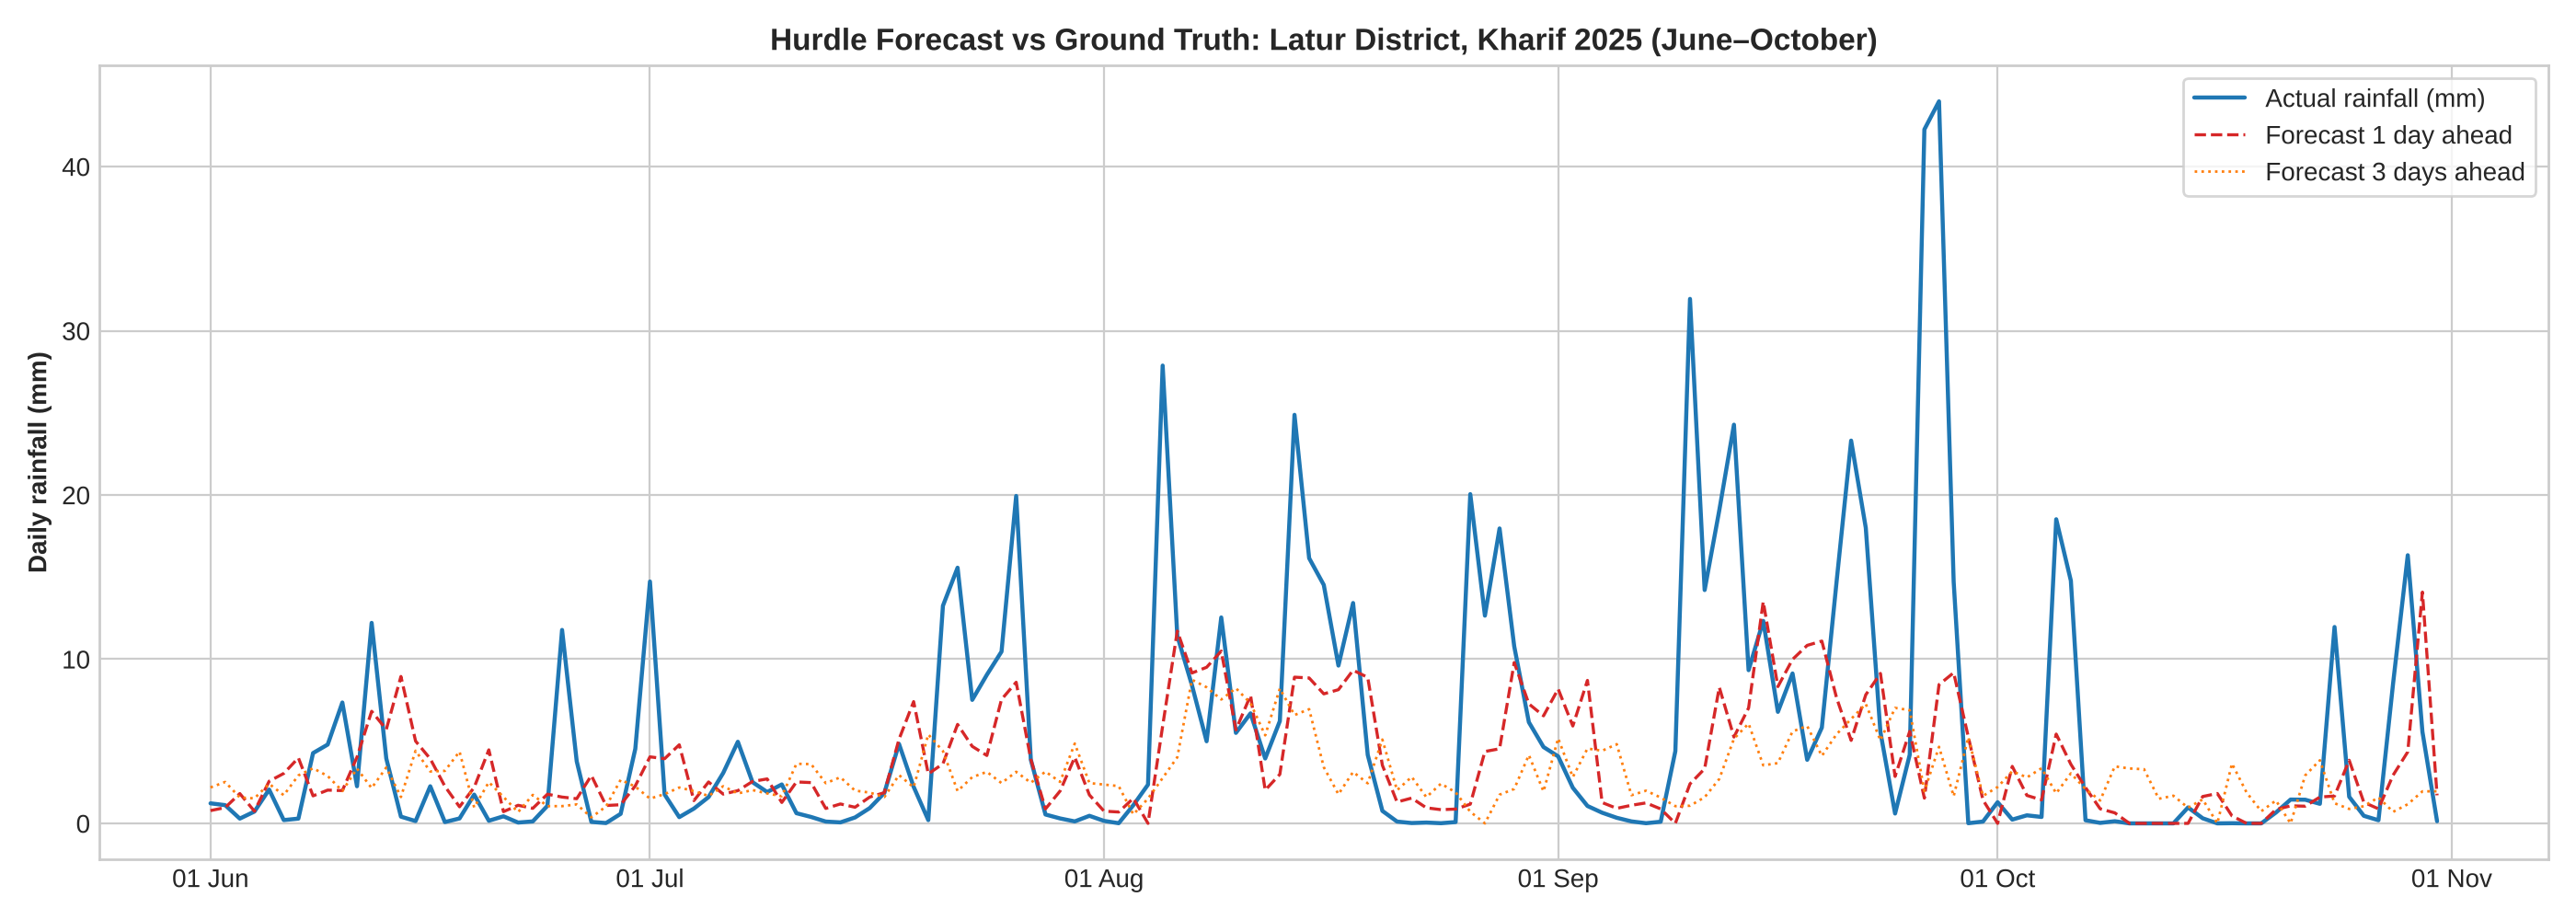
\includegraphics[width=\textwidth]{hurdle_latur_kharif2025.png}
	\caption{Hurdle model, Latur, Kharif 2025: forecasts one and three days ahead against observed rainfall.}
	\label{fig:hurdlelatur}
\end{figure}

What the model is good for in this system follows from these numbers. It gives a reliable short-range picture of whether the next one to three days are likely to stay dry, which is what decides whether a dry spell is continuing. Its gate also produces a \emph{probability of rain} that can be shown to users directly. It is not a season-long forecast; Stages 3--4 will combine it with the rainfall already observed in the season (Chapter~\ref{chap.conclusion}).

\section{Comparative study}
To test whether the hurdle model is the right choice, four other approaches were trained per district on the same weather data.

\subsection{LSTM network}
A Long Short-Term Memory network \cite{hochreiter1997long} reads a sequence one day at a time and keeps an internal memory, with gates that learn what to keep and what to forget. One model was trained per district.

\textbf{Inputs.} A window of the last 45 days, with 19 features per day: the 11 raw variables (rainfall, mean/maximum/minimum temperature, relative humidity, wind speed at 2\,m and 50\,m, surface pressure, solar radiation, dew point, cloud cover) and 8 rolling features (rainfall totals over 7, 14 and 30 days; 7-day means of humidity, solar radiation, wind, wind at 50\,m and cloud cover), plus day-of-year sine/cosine. Rainfall and wind speed were log-transformed, and all values scaled using the training period only.

\textbf{Architecture and training.} One LSTM layer of 128 units, followed by dense layers of 384 and 192 units with dropout 0.25, producing all 11 variables for the next 3 days in one output (33 numbers). Training used the Huber loss \cite{huber1964robust}, which behaves like squared error for small mistakes and like absolute error for large ones,
\begin{equation}
	\mathcal{L}_\delta(y,\hat{y}) =
	\begin{cases}
		\tfrac{1}{2}(y-\hat{y})^2 & \text{if } |y-\hat{y}| \le \delta,\\
		\delta\,|y-\hat{y}| - \tfrac{1}{2}\delta^2 & \text{otherwise,}
	\end{cases}
\end{equation}
with the Adam optimiser \cite{kingma2015adam} (learning rate $5\times10^{-4}$, batch size 16) and early stopping after 12 epochs without validation improvement. The data were split into training (to 2018), validation (2019--2021) and test (2022 onward). Figure~\ref{fig:loss} shows the loss curves for Latur.

\begin{figure}[H]
	\centering
	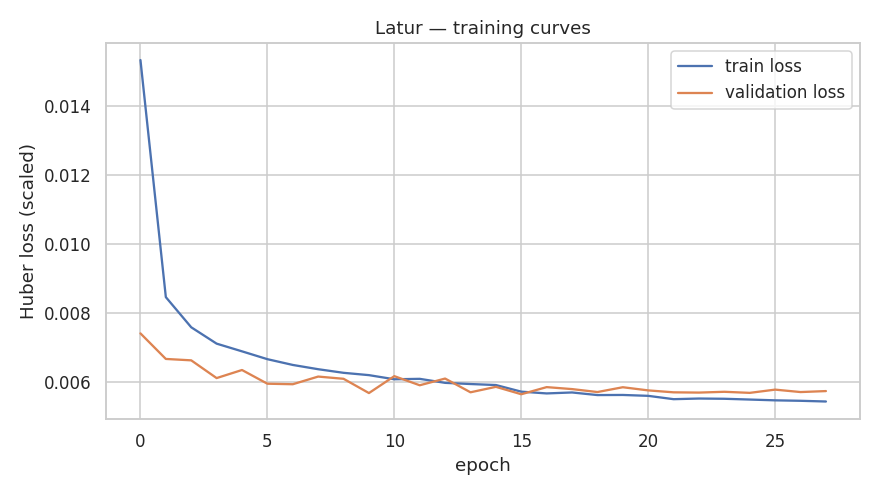
\includegraphics[width=0.65\textwidth]{loss_curve.png}
	\caption{Comparative LSTM: training and validation loss for Latur.}
	\label{fig:loss}
\end{figure}

\textbf{Results.} Because the LSTM forecasts all 11 variables, it also shows how forecastable the other variables are (Figure~\ref{fig:heatmap}, Table~\ref{tab:lstmdistrict}). Smooth variables are forecast well: temperature, humidity and dew point reach $R^2$ of 0.85--0.94 in every district. Rainfall is by far its weakest variable ($R^2$ 0.10--0.22): as Figures~\ref{fig:parity} and~\ref{fig:samples} show, its rainfall forecasts are squeezed towards small values and heavy rain is missed, exactly the behaviour described in Section~5.2.

\begin{figure}[H]
	\centering
	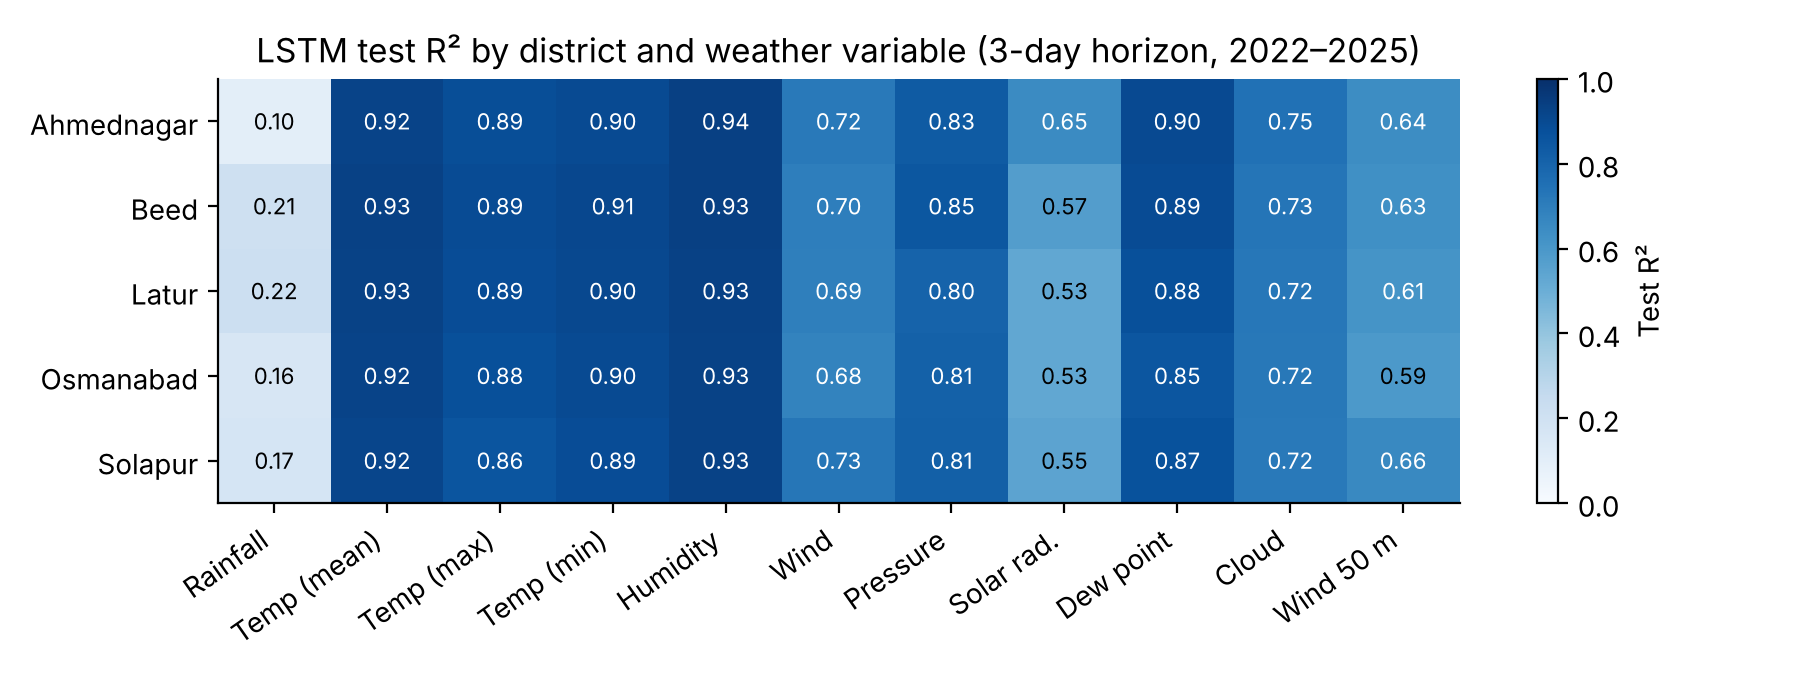
\includegraphics[width=\textwidth]{lstm_r2_heatmap.png}
	\caption{Comparative LSTM: test $R^2$ for every district and variable.}
	\label{fig:heatmap}
\end{figure}

\begin{table}[H]
	\centering
	\caption{Comparative LSTM: test results per district (2022 onward)}
	\label{tab:lstmdistrict}
	\begin{tabular}{lccc}
		\toprule
		\textbf{District} & \textbf{Average $R^2$ (11 variables)} & \textbf{Rainfall $R^2$} & \textbf{Rainfall MAE (mm)} \\
		\midrule
		Ahmednagar & 0.749 & 0.101 & 1.67 \\
		Beed & 0.750 & 0.209 & 1.68 \\
		Latur & 0.738 & 0.218 & 1.92 \\
		Osmanabad & 0.725 & 0.163 & 1.98 \\
		Solapur & 0.736 & 0.169 & 1.68 \\
		\bottomrule
	\end{tabular}
\end{table}

\begin{figure}[H]
	\centering
	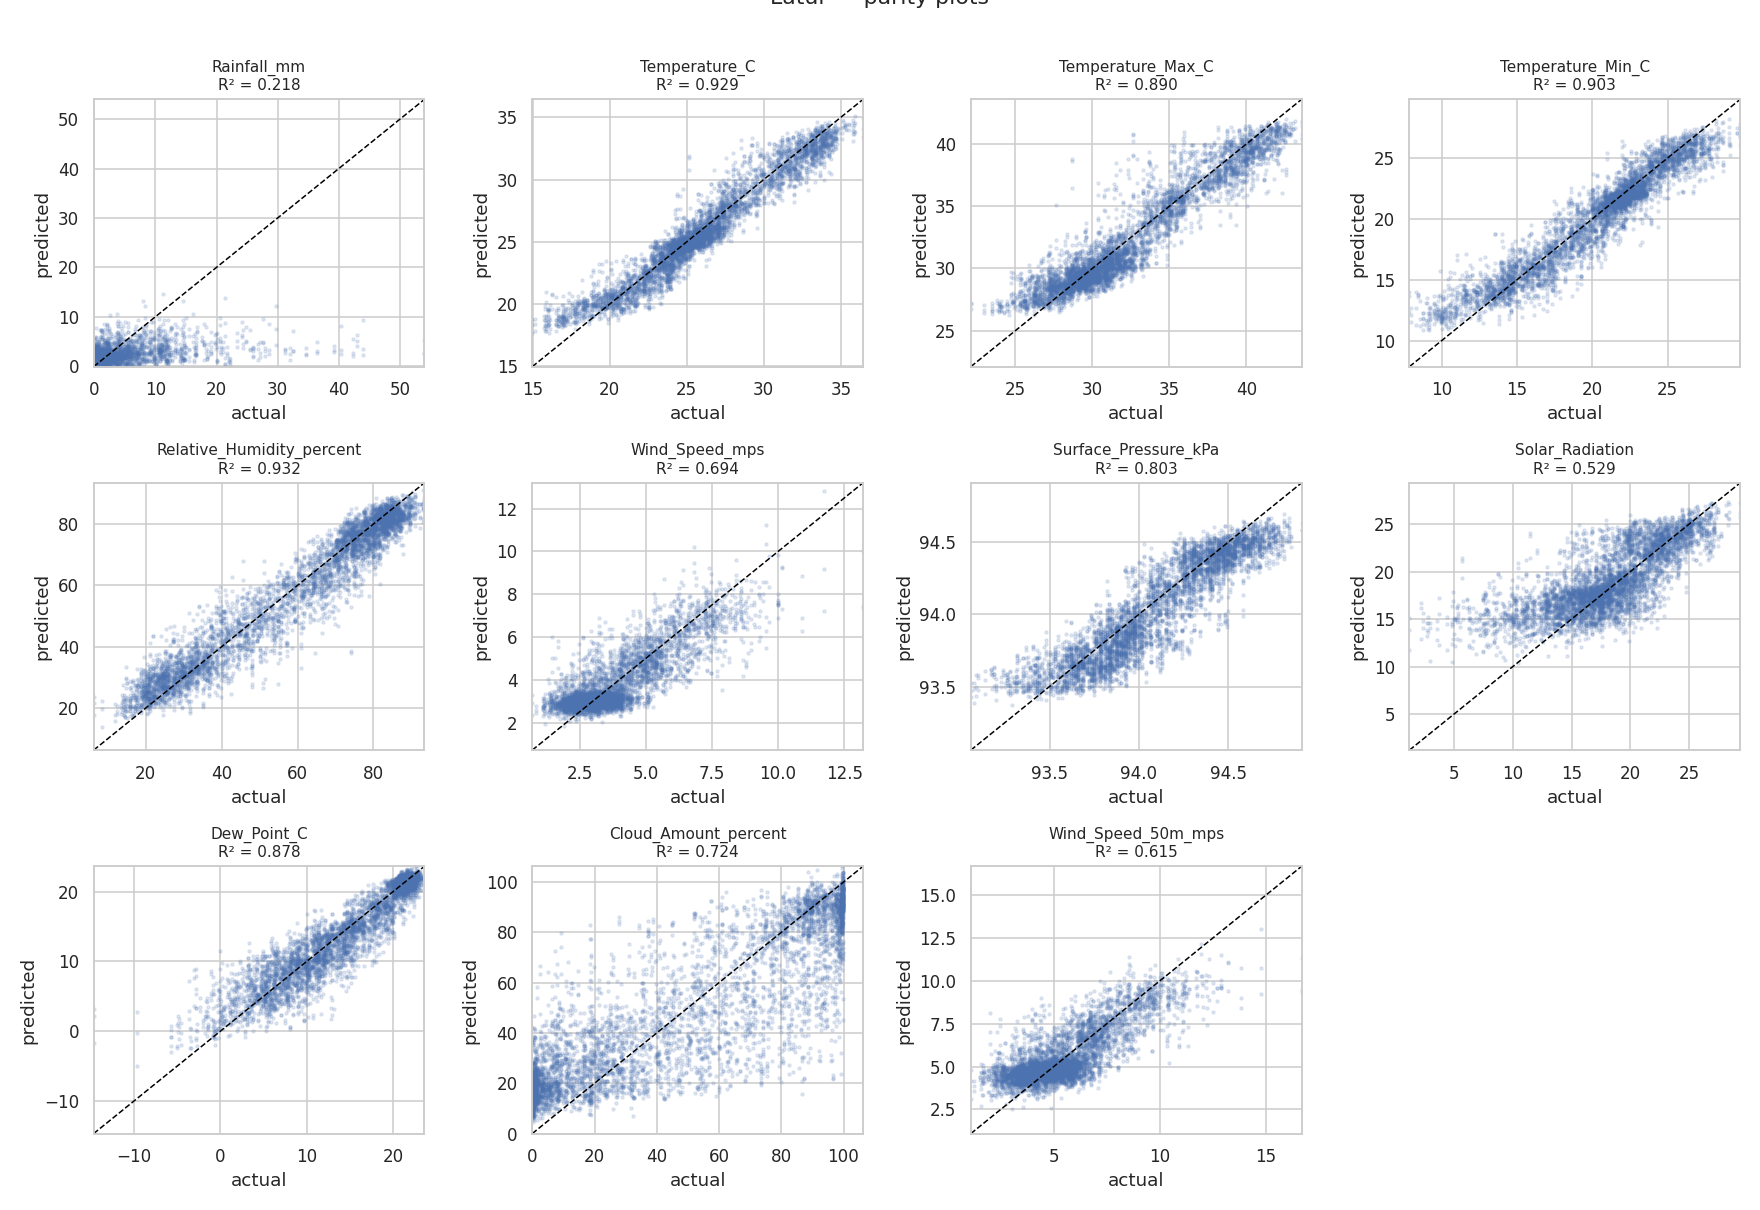
\includegraphics[width=0.9\textwidth]{parity_plots.png}
	\caption{Comparative LSTM, Latur: predicted against observed values on the test set. Temperature and humidity lie close to the diagonal; rainfall forecasts are compressed towards small values.}
	\label{fig:parity}
\end{figure}

\begin{figure}[H]
	\centering
	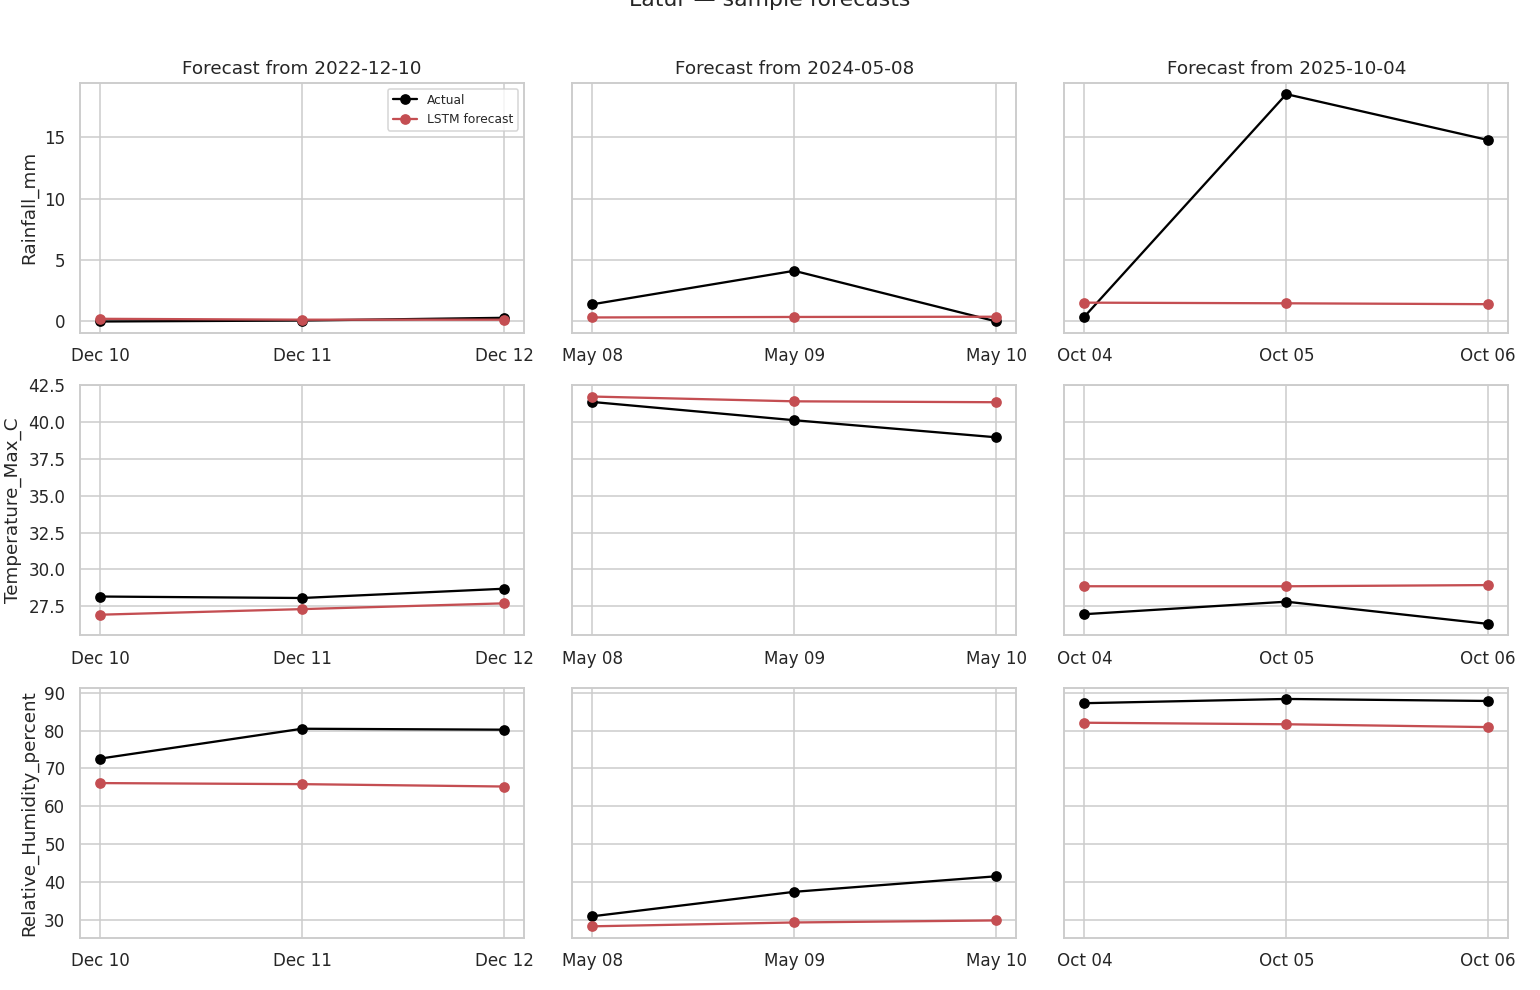
\includegraphics[width=0.9\textwidth]{sample_forecasts.png}
	\caption{Comparative LSTM, Latur: three sample 3-day forecasts. Temperature and humidity follow the observed trend; the heavy rain of 5--6 October 2025 is missed.}
	\label{fig:samples}
\end{figure}

\subsection{SARIMA}
A seasonal ARIMA model \cite{box2015time} was fitted per district as the statistical baseline. It forecasts the next value as a linear function of recent values, recent errors and the values one season earlier. It captures regular seasonality but assumes linear relations, so it struggles with the abrupt on/off behaviour of daily rain.

\subsection{XGBoost}
An XGBoost model \cite{chen2016xgboost} was trained per district on lagged and rolling-window weather features and seasonal terms. Gradient-boosted trees capture non-linear interactions, but used as a single regressor XGBoost treats rainfall as one continuous quantity and does not separate "will it rain?" from "how much?". The hurdle model uses the same family of learners but splits the problem in two.

\subsection{Temporal Fusion Transformer}
The TFT \cite{lim2021temporal} was trained as a multivariate, multi-horizon forecaster with attention over past time steps and learnt input selection. It is the most complex model in the study, and with about 9,500 daily rows per district it has comparatively little data to learn from. Like the LSTM, it predicts rainfall as a continuous value and has no explicit treatment of dry days.

\section{Comparison of results}
\subsection{Hurdle model and LSTM under the same protocol}
The LSTM and the hurdle model were both evaluated as genuine forecasts on the same test period (2022 onward), so their rainfall results can be compared directly (Table~\ref{tab:compare}, Figure~\ref{fig:rainskill}).

\begin{table}[H]
	\centering
	\caption{Rainfall test $R^2$: main hurdle model vs comparative LSTM}
	\label{tab:compare}
	\begin{tabular}{lccccc}
		\toprule
		& \multicolumn{4}{c}{\textbf{Hurdle (main)}} & \textbf{LSTM} \\
		\cmidrule(lr){2-5}
		\textbf{District} & \textbf{Day +1} & \textbf{Day +2} & \textbf{Day +3} & \textbf{Mean} & \textbf{Days +1..+3} \\
		\midrule
		Ahmednagar & 0.151 & 0.103 & 0.072 & 0.109 & 0.101 \\
		Beed & 0.259 & 0.190 & 0.147 & 0.199 & 0.209 \\
		Latur & 0.289 & 0.186 & 0.154 & 0.210 & 0.218 \\
		Osmanabad & 0.261 & 0.173 & 0.134 & 0.189 & 0.163 \\
		Solapur & 0.282 & 0.150 & 0.106 & 0.179 & 0.169 \\
		\bottomrule
	\end{tabular}
\end{table}

\begin{figure}[H]
	\centering
	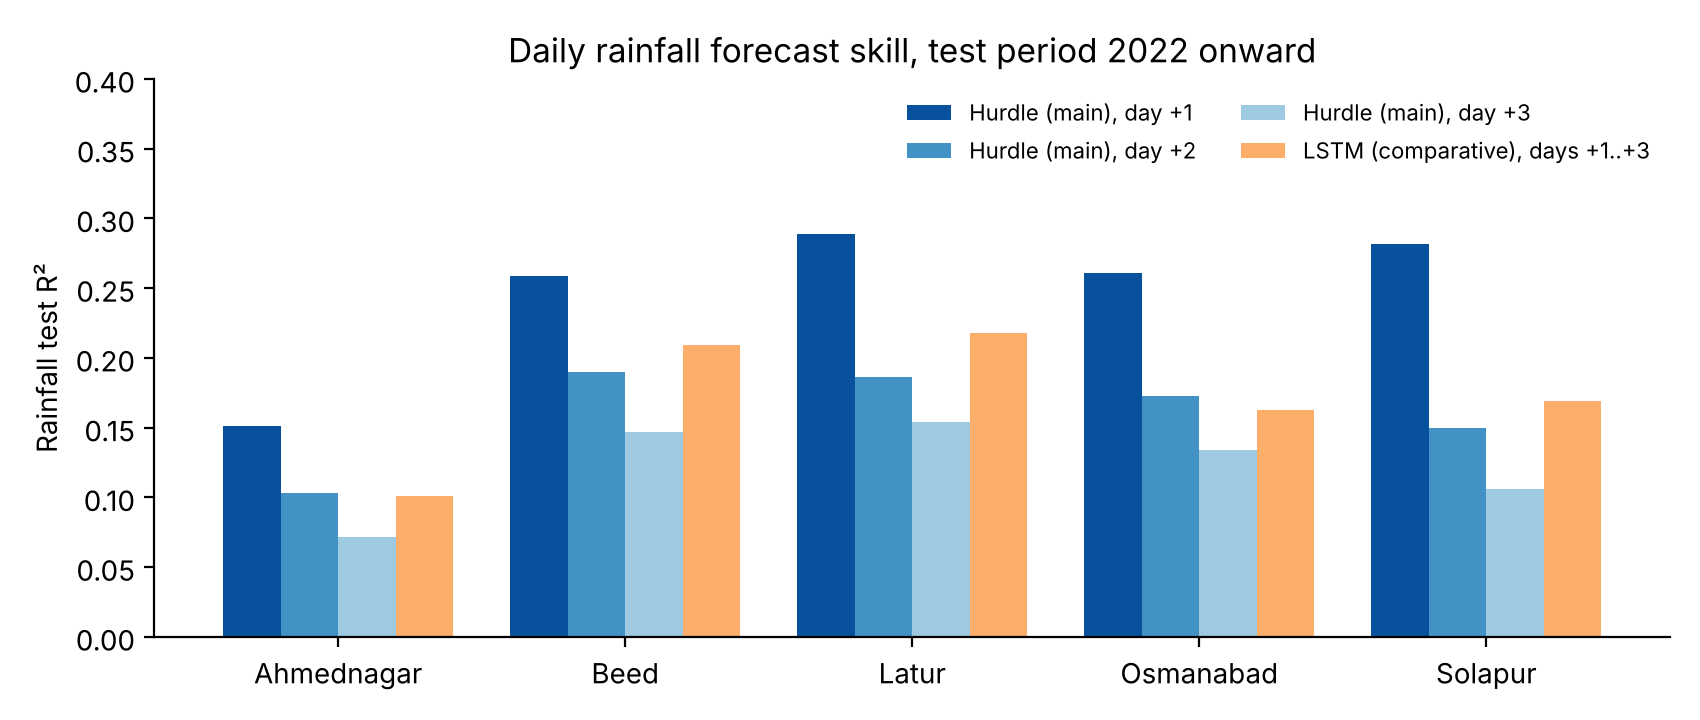
\includegraphics[width=0.9\textwidth]{rain_skill.png}
	\caption{Daily rainfall forecast skill of the main hurdle model at each horizon, compared with the LSTM.}
	\label{fig:rainskill}
\end{figure}

One day ahead, the hurdle model is better than the LSTM's rainfall forecast in every district. Averaged over the three days the two are close: the hurdle model is ahead in three districts and slightly behind in Beed and Latur.

\subsection{All five models as presented at the first review}
Table~\ref{tab:review} reproduces the test $R^2$ values presented at the first review. These numbers come from each model's own experimental set-up and are \textbf{not directly comparable}: the LSTM column averages all 11 variables (most of which are easy), the hurdle column is from the first, same-day version described in Section~\ref{sec:leak}, and the models differ in splits, targets and scaling. They are shown for completeness. Re-running SARIMA, XGBoost and TFT under the same protocol as Table~\ref{tab:compare} is part of the second-phase plan.

\begin{table}[H]
	\centering
	\caption{Test $R^2$ of the five models as presented at the first review (individual set-ups)}
	\label{tab:review}
	\begin{tabular}{lccccc}
		\toprule
		\textbf{District} & \textbf{Hurdle$^b$} & \textbf{SARIMA} & \textbf{XGBoost} & \textbf{LSTM$^a$} & \textbf{TFT} \\
		\midrule
		Ahmednagar & 0.923 & 0.432 & 0.303 & 0.749 & 0.511 \\
		Beed & 0.940 & 0.479 & 0.506 & 0.750 & 0.439 \\
		Latur & 0.945 & 0.592 & 0.590 & 0.738 & 0.500 \\
		Osmanabad & 0.885 & 0.544 & 0.549 & 0.725 & 0.439 \\
		Solapur & 0.787 & 0.512 & 0.509 & 0.736 & 0.372 \\
		\bottomrule
	\end{tabular}
	\\[2pt]
	\footnotesize $^a$ Average over all 11 variables. \quad $^b$ First (same-day) version; superseded by Table~\ref{tab:hurdle}.
\end{table}

\section{Why the hurdle model is the main model}
\begin{enumerate}
	\item \textbf{It is built for rainfall.} It separates "will it rain?" from "how much?", which matches how daily rainfall actually behaves (Section~5.2). None of the comparative models does this.
	\item \textbf{It gives the better next-day rainfall forecast} of the two models evaluated under the same protocol, in all five districts, and is on par with the LSTM over three days.
	\item \textbf{Its output is directly useful.} Besides the amount, the gate gives a probability of rain and a forecast of exactly 0\,mm on dry days, and it separates dry from rainy days correctly 81--88\% of the time up to three days ahead. This is what the dry-spell and onset rules in Stages 3--4 need.
	\item \textbf{It is light and easy to maintain.} It trains quickly on an ordinary CPU without a GPU, and is simple to version, retrain and monitor; it is the model run in the MLOps pipeline (Chapter~\ref{chap.7}).
	\item \textbf{It is easier to explain.} Gradient-boosted trees work with SHAP-style explanations \cite{lundberg2017unified}, which the project already plans for the yield stage.
\end{enumerate}
The comparative study remains useful: the LSTM shows that temperature, humidity and dew point can be forecast three days ahead with high accuracy, and these variables are available as supporting inputs if a later stage needs them.

\section{Summary}
A per-district, per-horizon two-stage hurdle model is the main forecasting model of the project. It forecasts daily rainfall 1--3 days ahead using only information available on the forecast day, with test $R^2$ of 0.15--0.29 one day ahead, falling to 0.07--0.15 at three days; its rain gate classifies 81--88\% of days correctly as dry or rainy. It gives better next-day rainfall forecasts than the LSTM, the comparative model evaluated under the same protocol. A comparative study of LSTM, SARIMA, XGBoost and TFT confirmed that models treating rainfall as a single continuous value struggle with its many dry days and rare heavy events, while the LSTM forecasts smoother variables such as temperature and humidity very well.

\chapter{Knowledge Graph from the Contingency Plans}
\label{chap.6}
\section{Why a knowledge graph}
The contingency plans contain exactly the guidance the system must give, but in a form a computer cannot use: tables of free text spread over 30 to 50 pages, with different layouts in different plans. The recommendations also depend on several things at once. The right action for a delayed monsoon depends on the district, the crop, the soil, the season and sometimes the crop stage, and soil types and crops are shared between districts.

A knowledge graph stores such facts as nodes (things) joined by typed edges (relations). It answers multi-hop questions that a flat lookup table cannot, for example "which past seasons in Beed had the same mid-season dry spell, and what soybean yield followed?", and it can keep, on every edge, the plan page the fact came from. The graph needs no data beyond what the preprocessing already produces, and at under a thousand nodes it is small enough to run in memory with NetworkX \cite{hagberg2008exploring} and to export to a graph database such as Neo4j.

\section{Build pipeline}
The graph is built by five scripts, run in order by \texttt{run\_all.py}:

\begin{table}[H]
	\centering
	\caption{Knowledge-graph build steps}
	\label{tab:kgsteps}
	\small
	\begin{tabularx}{\textwidth}{clY}
		\toprule
		\textbf{Step} & \textbf{Script} & \textbf{Output} \\
		\midrule
		1 & \texttt{extract\_pdfs.py} & District profile table; 1,063 condition$\to$action rows; 27 "not applicable" statements \\
		2 & \texttt{label\_seasons.py} & 124 condition labels for past seasons; weather summary for all 260 district-seasons \\
		3 & \texttt{build\_graph.py} & The graph, saved as JSON and GraphML, with summary statistics \\
		4 & \texttt{build\_html\_viewer.py} & An interactive viewer that opens in any browser \\
		5 & \texttt{export\_neo4j.py} & One CSV per node and relation type plus an \texttt{import.cypher} script \\
		\bottomrule
	\end{tabularx}
\end{table}

\section{Extracting the contingency tables}
The extractor uses pdfplumber to read the tables page by page. The plans follow a common ICAR template but are not uniform, so the extractor reads each table's own header instead of assuming fixed columns. The main difficulties and how they were handled:

\begin{itemize}
	\item \textbf{Different column meanings by table type.} Delayed-onset tables have \emph{change in crop / agronomic measures / remarks}; normal-onset and mid-season tables have \emph{crop management / soil nutrient and moisture conservation / remarks}; terminal-drought tables have \emph{crop management / Rabi crop planning / remarks}; and the unusual-rain, flood and extreme-event tables have one column per crop stage (vegetative, flowering, maturity, post-harvest).
	\item \textbf{Wide and two-row headers.} Solapur's tables have 8 to 11 columns with spanned header cells, which are inherited from the left; its \emph{Kharif $|$ Rabi} sub-columns become separate rows, each with its own season. Beed uses two header rows; each column takes its role from whichever row names it.
	\item \textbf{Page breaks.} Text that spills onto the next page is appended to the row it belongs to, and split phrases such as "Delay by 4 weeks" + "2nd week of July" are re-joined.
	\item \textbf{Irrigated situations} (canal, tank, groundwater shortages) are given their own category instead of inheriting the drought heading printed above them.
	\item \textbf{Crop names inside free text,} e.g.\ "Kharif Pearlmillet Preseasonal sugarcane Maize", are found by scanning against the crop vocabulary; a "Rabi" or "Kharif" prefix sets the season.
	\item \textbf{"-do-" and "As above"} cells are resolved from the row above in the same column, and every resolution is recorded. Five dittos have nothing above them and are left flagged.
\end{itemize}

\textbf{Accuracy check.} The first 20 characters of every extracted field were searched for in the cells of the page it came from: of 4,027 fields, 99\% were found verbatim, and the rest are the deliberate joins described above. Beed page 19 and Solapur page 11 were also compared visually with the PDF.

Each recommendation also needs a season. It is taken, in order of preference, from the PDF text itself ("Rabi sorghum", or a Kharif/Rabi sub-column), from the crop calendar for single-season crops (Soybean $\to$ Kharif, Gram $\to$ Rabi), or from the fact that Section~2.1.1 rainfed drought tables concern the Kharif monsoon. Where none applies the season is marked \emph{unspecified}, and such rows are still returned by queries rather than silently dropped.

\section{Season labeller}
\label{sec:labeller}
To connect the plans with real history, every past district-season from 2000 to 2025 is labelled with the conditions it actually experienced, using the plans' own definitions applied to the observed daily rainfall (Table~\ref{tab:labeller}).

\begin{table}[H]
	\centering
	\caption{Rules used by the season labeller}
	\label{tab:labeller}
	\small
	\begin{tabularx}{\textwidth}{p{4.3cm}Y}
		\toprule
		\textbf{Label} & \textbf{Rule} \\
		\midrule
		Onset delayed 2/4/6/8 weeks & Onset = first day from 1 June with a 3-day total $\ge$ 20 mm and no run of $\ge$ 14 rainless days ($<$ 2.5 mm) in the next 30 days. Delay is counted in weeks after 8 June, because the plans equate a 2-week delay with the 4th week of June. \\
		Normal onset, then dry spell & Onset not delayed, and a run of $\ge$ 15 rainless days starting within 30 days of onset. \\
		Mid-season dry spell (vegetative / flowering) & A run of $\ge$ 14 rainless days starting 31--60 / 61--90 days after onset. \\
		Terminal drought & Rainfall from 15 September to 15 October below 50\% of the district's own 2000--2025 mean for that window. \\
		Continuous high rainfall & A 3-day total $\ge$ 150 mm (Kharif), or $\ge$ 64.5 mm in November--February (unseasonal, Rabi). \\
		\bottomrule
	\end{tabularx}
\end{table}

The labeller found 124 condition labels across the 260 district-seasons (Figure~\ref{fig:labels}). The labels agree with known bad years: terminal drought appears in 2014 and 2018, the onset is delayed by about 8 weeks in 2000 and 2015, and Solapur's onset is delayed in 2012. For Beed, for example, 2018 is labelled \emph{normal onset followed by a 25-day dry spell} and \emph{terminal drought} (only 29.7 mm between 15 September and 15 October against a district mean of 141.1 mm), and that season's Kharif rainfall was 37\% below the mean.

\begin{figure}[H]
	\centering
	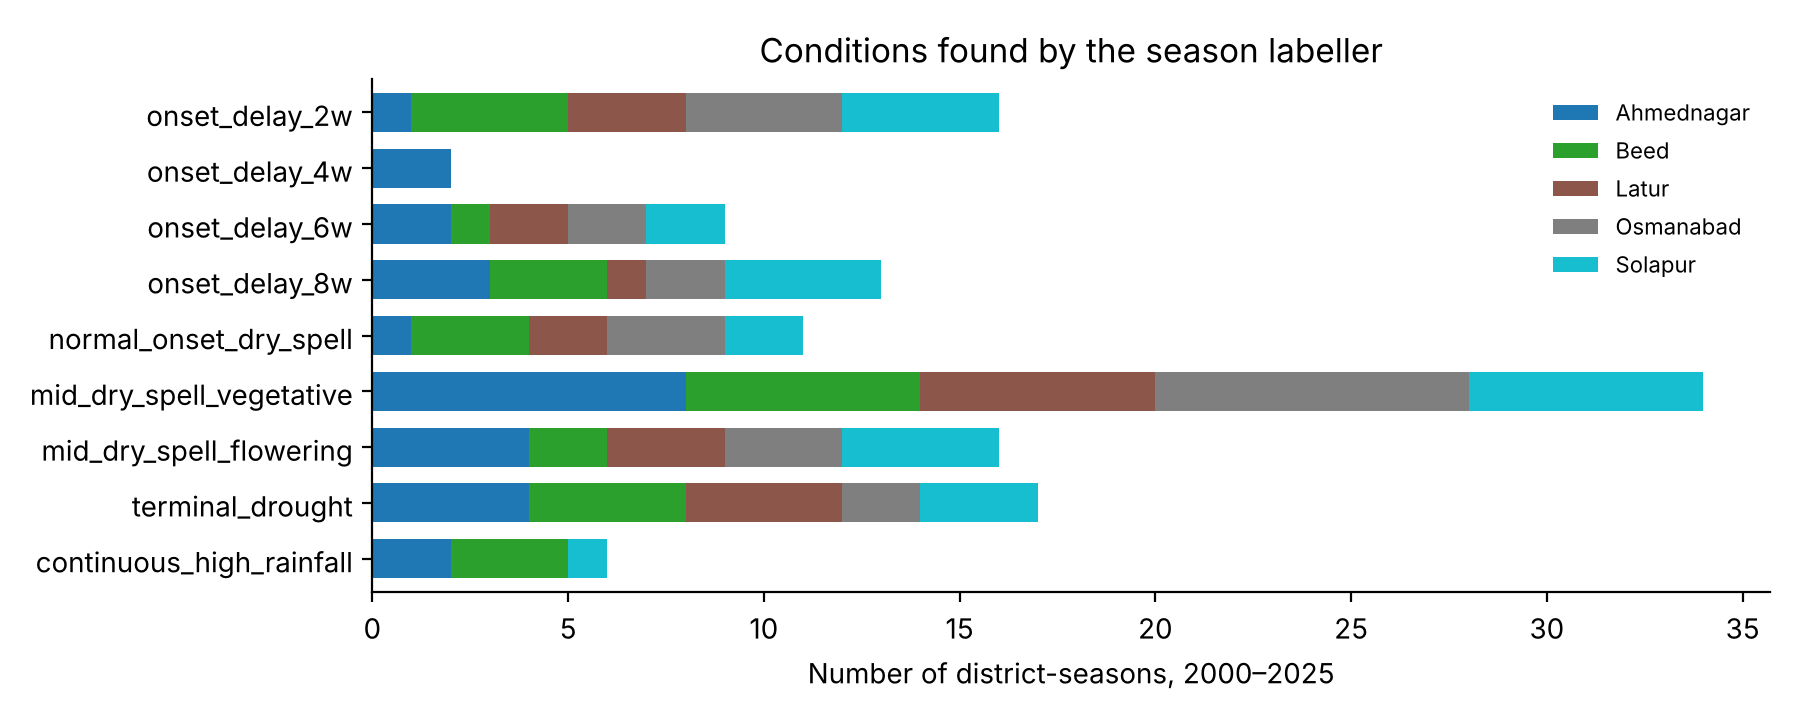
\includegraphics[width=\textwidth]{season_labels.png}
	\caption{Number of district-seasons, 2000--2025, labelled with each condition. Mid-season dry spells during vegetative growth are the most common.}
	\label{fig:labels}
\end{figure}

The labeller is a transparent first version, not a validated drought index, and it also acts as a stand-in for Stage~4: when Stage~4 is built, it will write a file with the same columns and the graph will use it without any change to its schema.

\section{Graph schema}
The finished graph has \textbf{833 nodes} of nine types and \textbf{4,353 edges} of fifteen relation types (Tables~\ref{tab:nodes} and~\ref{tab:edges}).

\begin{table}[H]
	\centering
	\caption{Node types}
	\label{tab:nodes}
	\small
	\begin{tabularx}{\textwidth}{lrY}
		\toprule
		\textbf{Type} & \textbf{Count} & \textbf{What it represents} \\
		\midrule
		District & 5 & The district, with its rainfall normal and irrigated share from the plan \\
		SoilType & 12 & Soil categories from the plans (e.g.\ medium-deep black soil) \\
		Season & 2 & Kharif, Rabi \\
		Crop & 35 & 5 core, 4 extended, 26 fallback/horticulture crops named in the plans \\
		Condition & 7 & Early-season, mid-season and terminal drought; irrigated water shortage; unusual rains; floods; extreme events \\
		ConditionDetail & 24 & Precise sub-types with machine-readable values, e.g.\ onset delayed 4 weeks, 2-week dry spell at flowering, hailstorm \\
		Action & 462 & Unique recommendation texts, split into the plan's own columns \\
		Year & 26 & 2000 to 2025 \\
		SeasonRecord & 260 & One per district, season and year, with that season's weather summary \\
		\bottomrule
	\end{tabularx}
\end{table}

\begin{table}[H]
	\centering
	\caption{Main relation types}
	\label{tab:edges}
	\small
	\begin{tabularx}{\textwidth}{llrY}
		\toprule
		\textbf{Relation} & \textbf{From $\to$ To} & \textbf{Count} & \textbf{Meaning} \\
		\midrule
		RECOMMENDS & ConditionDetail $\to$ Action & 1,063 & One per plan table row; carries district, crop, season, soil, crop stage and \textbf{source page} \\
		APPLIES\_TO\_CROP & Crop $\to$ Action & 702 & The action is for this crop \\
		SOIL\_CONTEXT & SoilType $\to$ Action & 399 & The action is for this soil \\
		SUGGESTS\_CROP & Action $\to$ Crop & 321 & An alternative or Rabi follow-up crop named in the action \\
		HAD\_YIELD & SeasonRecord $\to$ Crop & 788 & The DES area, production and yield that season \\
		EXPERIENCED & SeasonRecord $\to$ ConditionDetail & 124 & The condition the season actually had (from the labeller) \\
		GROWS & District $\to$ Crop & 84 & The district grows this crop \\
		NOT\_APPLICABLE & District $\to$ Condition & 27 & The plan rules this condition out (e.g.\ floods in Beed) \\
		HAS\_SOIL & District $\to$ SoilType & 15 & With area and share \\
		\bottomrule
	\end{tabularx}
	\\[2pt]
	\footnotesize Others: SUBTYPE\_OF (24), IN\_SEASON (20), INCLUDES (6), HAS\_SEASON\_RECORD, IN\_YEAR and OF\_SEASON (260 each).
\end{table}

The core of the graph is the path
\[
\text{Condition} \leftarrow \text{ConditionDetail} \xrightarrow{\text{RECOMMENDS}} \text{Action} \leftarrow \text{Crop},\ \text{SoilType}
\]
filtered by the district and season stored on each RECOMMENDS edge. Around it, the SeasonRecord nodes link the official guidance to 26 years of observed history and yield. Figure~\ref{fig:kgview} shows the interactive viewer.

\begin{figure}[H]
	\centering
	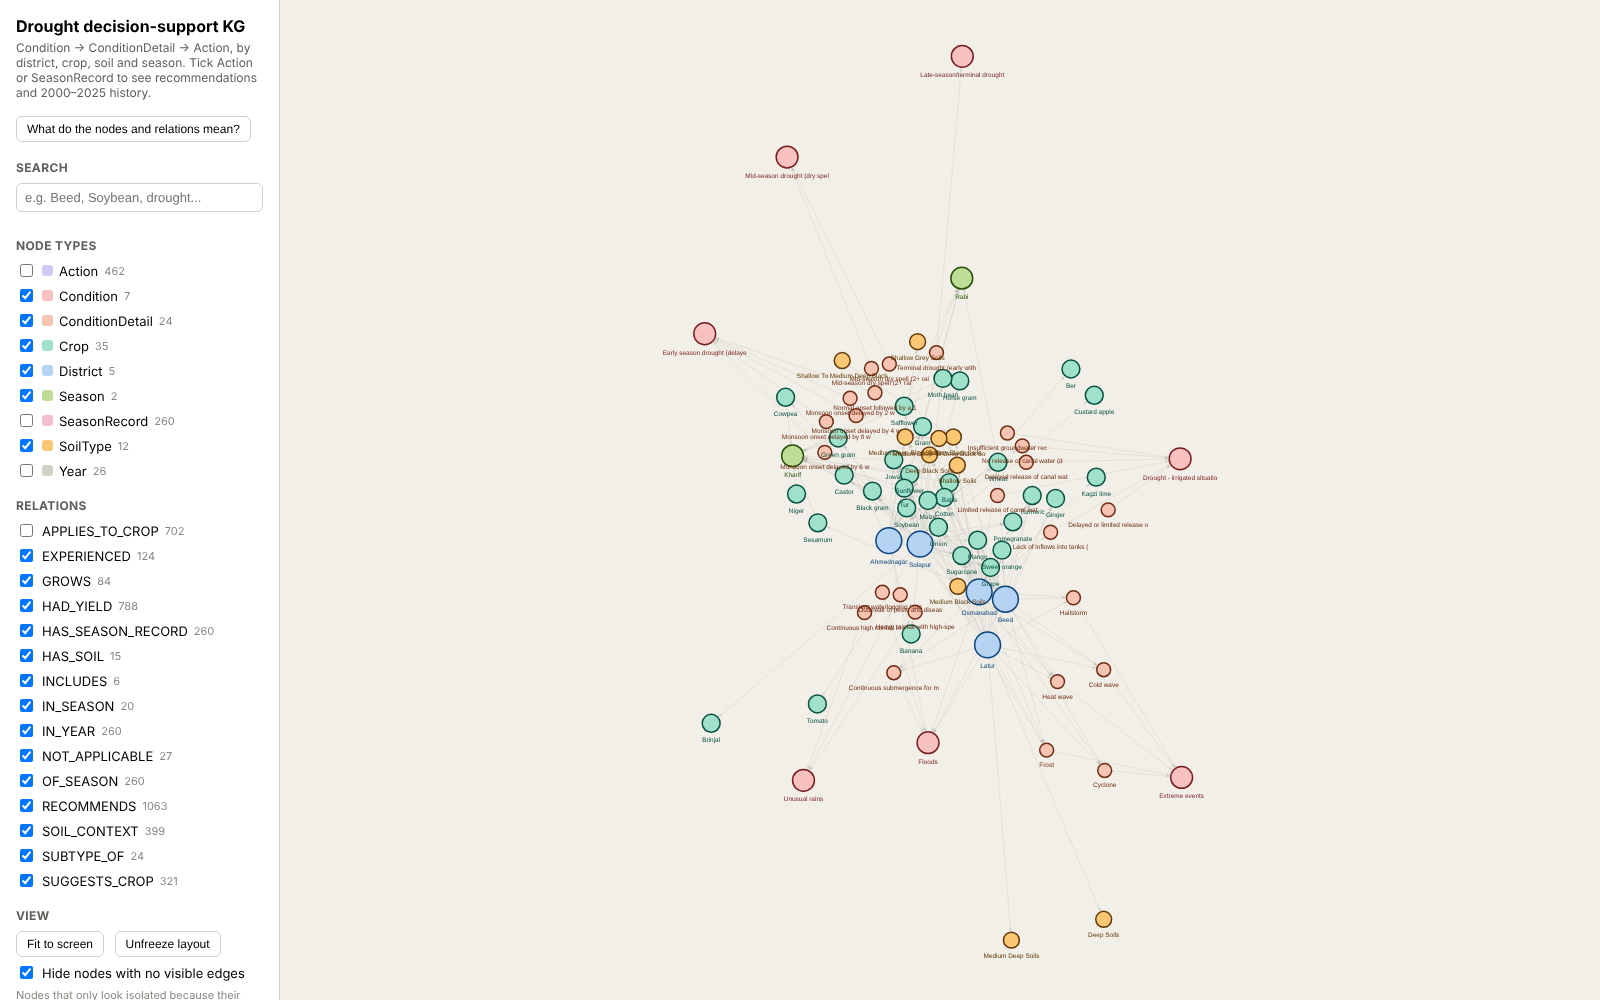
\includegraphics[width=\textwidth]{kg_viewer.png}
	\caption{The interactive knowledge-graph viewer. Node types and relations can be switched on and off in the sidebar; clicking a node or edge shows its details and source. Actions and season records are hidden by default for readability.}
	\label{fig:kgview}
\end{figure}

\section{Querying the graph}
\texttt{kg\_query.py} provides query functions (\texttt{recommend}, \texttt{alternatives}, \texttt{not\_applicable}, \texttt{district\_profile}, \texttt{season\_history}, \texttt{similar\_seasons}, \texttt{yield\_baseline}) and one combined call designed for the LLM layer:

\begin{center}
\texttt{retrieve\_context(G, district, crop, season, condition)}
\end{center}

It returns a single JSON-ready bundle containing the condition's definition, the district profile, the official recommendations with page citations, alternative crops, past seasons with the same condition and the yields that followed, the all-years yield baseline, the plan's "not applicable" statements, and the guardrail text the LLM must obey. The condition can be given as a detail code (\texttt{onset\_delay\_4w}), a category code (\texttt{mid\_season\_drought}) or a category name.

\subsection{Worked example}
For \emph{Beed, Soybean, Kharif}, the graph returns, among others, the following recommendations from the Beed plan:

\begin{table}[H]
	\centering
	\caption{Selected Beed recommendations for soybean returned by the graph}
	\label{tab:example}
	\small
	\begin{tabularx}{\textwidth}{p{4.2cm}Yc}
		\toprule
		\textbf{Condition} & \textbf{Recommended action} & \textbf{Page} \\
		\midrule
		Onset delayed 2 weeks (4th week of June) & No change in cropping & 9 \\
		Onset delayed 4 weeks (2nd week of July) & Soybean (JS-335, MAUS-71) + pigeon pea (BSMR-736, 853, BDN-708, 711) intercrop in 4:2 or 6:3 rows & 10 \\
		Onset delayed 6 weeks (4th week of July) & Shift to pearl millet + pigeon pea in 4:2 or 3:3 rows & 12 \\
		Onset delayed 8 weeks (2nd week of August) & Pearl millet or sunflower (e.g.\ Morden, SS-56, LSH-36) & 13--14 \\
		Normal onset then 15--20 day dry spell & Gap-fill with the same or a short-duration cultivar to keep at least 75\% plant population & 15 \\
		Mid-season dry spell, vegetative & Interculture for weeding and to create a soil mulch; re-sow if plant population is below 50\% & 17--18 \\
		Mid-season dry spell, flowering & Give protective irrigation with sprinkler & 18 \\
		Continuous high rainfall & Drain out excess water; after harvest, shift produce to a safe place and dry it & 24 \\
		\bottomrule
	\end{tabularx}
\end{table}

Alongside these, the graph returns Beed's soil profile (58.9\% shallow black soils, 16\% net irrigated) and the past Kharif seasons labelled with the same condition together with the soybean yield DES recorded for them. This is exactly the material the LLM will be allowed to use.

\section{Neo4j export}
\texttt{export\_neo4j.py} writes one CSV per node and relation type and an \texttt{import.cypher} script that loads them, giving every node a unique key. It can also push the graph directly into a running database. A Cypher query template for the GraphRAG step is included. The export has been generated but not yet loaded into a live Neo4j instance; this is planned together with the GraphRAG layer.

\section{Limitations}
\begin{itemize}
	\item \textbf{The plans date from 2011.} Soil, irrigation and rainfall-normal figures are a single snapshot; Ahmednagar's plan gives no soil percentages and Latur's net irrigated share is not captured.
	\item \textbf{Soil vocabularies differ} between a plan's profile section and its tables, so links between them are made only where names match exactly; several soil groups still need manual checking.
	\item \textbf{Some rows are not captured,} for example rows whose crop cell holds no recognised crop (grasses, tree plantations).
	\item \textbf{Mixed rotation cells} such as "Kharif fallow -- Rabi sorghum / safflower / sunflower" can tag a crop with the wrong season.
	\item \textbf{The labeller uses gridded rainfall,} which smooths extremes, so heavy-rain labels are conservative; it cannot detect pests, hail or canal releases, which therefore come only from the plans.
	\item \textbf{Yield links are missing} for Gram, Wheat, Cotton and Safflower, which are absent from the DES table used.
\end{itemize}

\section{Summary}
The five contingency plans have been converted into a knowledge graph of 833 nodes and 4,353 edges in which every recommendation keeps its source page. A season labeller ties 26 years of observed weather and DES yields to the plans' own condition definitions, and a single query call returns everything the LLM layer will need to give a grounded, cited answer.

\chapter{MLOps Pipeline}
\label{chap.7}
\section{Why MLOps}
A forecasting model trained once and left alone slowly goes stale: new weather arrives every day, the climate shifts (rainfall in all five districts has risen over the 26 years, Chapter~\ref{chap.3}), and nobody notices when accuracy drops. Sculley et al.\ \cite{sculley2015hidden} point out that in real machine-learning systems the model is a small part of the whole, and most of the effort goes into data handling, configuration, serving and monitoring. MLOps is the practice of treating those parts as carefully as the model. For this project it means four things: the data and models are versioned, there is one clearly marked production model per district, forecasts are served through a stable interface, and performance is checked automatically.

\section{Architecture}
Figure~\ref{fig:mlops} shows the flow. The pipeline is built around the project's main forecasting model, the per-district hurdle rainfall model; the comparative models are kept as research notebooks and are not served.

\begin{figure}[H]
\centering
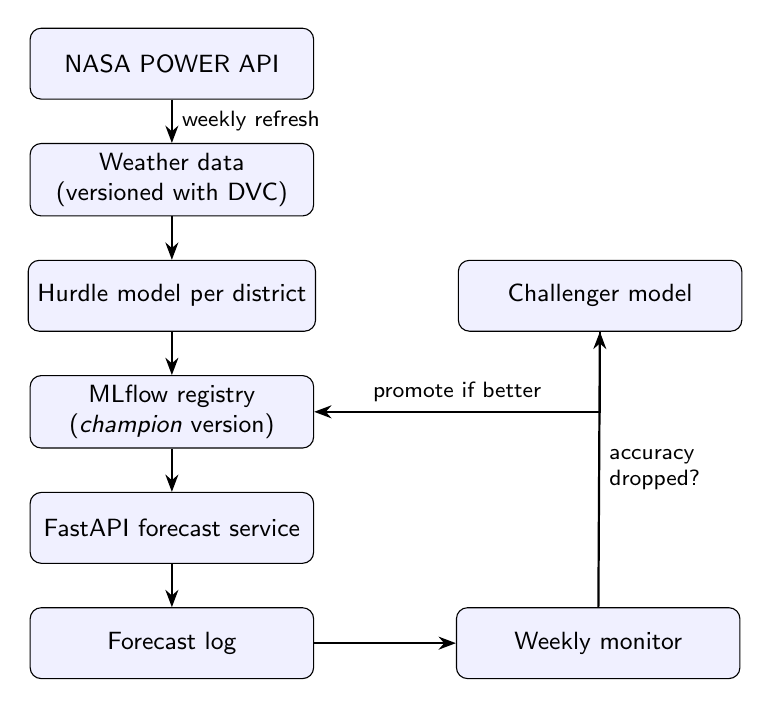
\begin{tikzpicture}[
  font=\sffamily\small,
  box/.style={draw, rounded corners, fill=blue!6, minimum width=3.6cm, minimum height=0.9cm, align=center},
  arr/.style={-{Stealth[length=2.2mm]}, thick}
]
\node[box] (n) {NASA POWER API};
\node[box, below=0.55cm of n] (d) {Weather data\\(versioned with DVC)};
\node[box, below=0.55cm of d] (m) {Hurdle model per district};
\node[box, below=0.55cm of m] (r) {MLflow registry\\(\emph{champion} version)};
\node[box, below=0.55cm of r] (a) {FastAPI forecast service};
\node[box, below=0.55cm of a] (l) {Forecast log};
\node[box, right=1.8cm of l] (mo) {Weekly monitor};
\node[box, right=1.8cm of m] (c) {Challenger model};
\draw[arr] (n) -- node[right, font=\sffamily\footnotesize]{weekly refresh} (d);
\draw[arr] (d) -- (m); \draw[arr] (m) -- (r); \draw[arr] (r) -- (a); \draw[arr] (a) -- (l);
\draw[arr] (l) -- (mo);
\draw[arr] (mo) -- node[right, font=\sffamily\footnotesize, align=left]{accuracy\\dropped?} (c);
\draw[arr] (c) |- node[pos=0.75, above, font=\sffamily\footnotesize]{promote if better} (r);
\end{tikzpicture}
\caption{MLOps flow for the forecasting stage}
\label{fig:mlops}
\end{figure}

\section{Components}
\begin{table}[H]
	\centering
	\caption{MLOps components}
	\label{tab:mlops}
	\small
	\begin{tabularx}{\textwidth}{p{3.4cm}p{4.2cm}Y}
		\toprule
		\textbf{Component} & \textbf{File / tool} & \textbf{What it does} \\
		\midrule
		Configuration & \texttt{params.yaml} & One place for districts, data paths, model settings (horizon 3, thresholds 0.25 mm and 0.35), split dates and monitoring thresholds \\
		Data refresh & \texttt{fetch\_nasa.py}, \texttt{clean.py} & Download the latest 60 days from NASA POWER and clean them into the weather folder \\
		Data versioning & DVC with a DagsHub remote & Keeps every version of the data and model outputs outside Git, with a small pointer file in Git \\
		Model pipeline & \texttt{hurdle\_pipeline.py} & Feature engineering, leakage-safe per-horizon training and evaluation, forecasting \\
		Registry & \texttt{registry.py}, MLflow & Logs each model with its parameters and metrics, versions it, and marks one version per district as the \emph{champion} \\
		Serving & \texttt{serve/app.py}, FastAPI, Docker & \texttt{/health} and \texttt{/forecast/\{district\}} endpoints; every forecast is appended to a log \\
		Monitoring & \texttt{monitor.py} & Scores logged forecasts against observed rain and, if accuracy has dropped, trains and tests a challenger \\
		Automation & GitHub Actions & CI tests on every push; weekly data refresh; weekly monitoring \\
		Tests & \texttt{pytest} & Check feature engineering and the hurdle model contract \\
		\bottomrule
	\end{tabularx}
\end{table}

\section{How it works}

\subsection{Data versioning}
The weather files are too large and change too often to keep in Git. DVC (Data Version Control) stores them in a remote store on DagsHub and keeps only a small pointer file in Git. Every model can therefore be traced to the exact data it was trained on, and any earlier state can be restored with \texttt{dvc pull}.

\subsection{Model registry and the champion}
MLflow \cite{zaharia2018accelerating} records every trained model together with its parameters (district, horizon, test start date, probability threshold) and test metrics. Each district has one registered model, \texttt{<district>\_hurdle}, with numbered versions. One version carries the alias \emph{champion}; the API always serves the champion, so switching to a better model means moving the alias rather than editing code.

\subsection{Serving}
The FastAPI service exposes \texttt{GET /health} and \texttt{GET /forecast/\{district\}}. On a request it fetches the district's champion from MLflow (and caches it), loads the latest weather, returns the forecast as JSON, and appends a line to \texttt{forecasts\_log.csv} with the model version, the date the forecast was made, the target date and the predicted rainfall.

\subsection{Automation}
Three GitHub Actions workflows run without manual effort:
\begin{itemize}
	\item \textbf{ci}: on every push or pull request, install the dependencies and run the tests;
	\item \textbf{weekly-data}: every Monday at 03:00 UTC (08:30 IST), pull the current data, fetch new NASA POWER data, clean it, push the new version to DVC and commit the updated pointer;
	\item \textbf{weekly-monitor}: every Monday at 06:00 UTC (11:30 IST), score the logged forecasts.
\end{itemize}

\subsection{Monitoring and champion--challenger promotion}
Once at least 30 days of logged forecasts can be compared with observed rainfall, the monitor computes RMSE and $R^2$ over the last 60 days. If $R^2$ has fallen more than 0.10 below the champion's recorded test $R^2$, it trains a \emph{challenger} on the latest data, evaluates both models on the same most recent year, and promotes the challenger only if it is better. This keeps a worse model from replacing a good one by accident.

\section{Current status and honest limitations}
\begin{itemize}
	\item The pipeline, registry, API, workflows and tests are in place and the five existing hurdle checkpoints have been registered.
	\item The registered checkpoints are the \emph{original} hurdle models, from the first, same-day version of the model (Section~\ref{sec:leak}). The API therefore labels its output \texttt{original\_checkpoint\_same\_day}. Registering the corrected three-horizon models described in Chapter~\ref{chap.5}, already implemented in \texttt{hurdle\_pipeline.py}, is the first task of the next phase.
	\item The monitor needs the forecast log to be versioned with DVC before the scheduled workflow can read it; this is a manual step today.
	\item The comparative models (LSTM, SARIMA, XGBoost, TFT) are not registered or served; if a later stage needs forecasts of other variables such as temperature, the LSTM can be added to the same pipeline.
\end{itemize}

\chapter{Conclusion and Scope for further Research}
\label{chap.conclusion}
\section{Conclusion of the first phase}
This thesis set out to build a decision-support system that links weather, crop yield, human impact and official guidance for five drought-prone districts of Maharashtra, with every recommendation traceable to the District Agriculture Contingency Plans. In the first phase the team:

\begin{enumerate}
	\item audited, cleaned and standardised four public data sources and documented their gaps;
	\item built the main forecasting model, a per-district two-stage hurdle model that forecasts daily rainfall one to three days ahead using only information available on the forecast day ($R^2$ 0.15 to 0.29 at one day, 0.07 to 0.15 at three days), after finding and correcting a data-leakage problem in its first version;
	\item carried out a comparative study with LSTM, SARIMA, XGBoost and TFT models; the hurdle model gave better next-day rainfall forecasts than the LSTM in every district, while the LSTM forecast temperature, humidity and dew point well ($R^2$ 0.85 to 0.94);
	\item turned the five contingency plans into a knowledge graph of 833 nodes and 4,353 edges, with 1,063 cited recommendations, 26 years of labelled season history and DES yields, and a single query call for the LLM layer; and
	\item set up an MLOps pipeline with data versioning, a model registry, a forecast API, weekly data refresh and monitoring with champion--challenger promotion.
\end{enumerate}

Three of the ten stages (selection, forecasting and knowledge-graph retrieval) are complete, and the interfaces between stages are fixed, so the remaining stages can be built in parallel and plugged in.

\section{Scope for further research: plan for the second phase}
The second phase completes the remaining seven stages and turns the components into one working system. The plan below follows the pipeline order.

\subsection{Strengthening the forecasting stage}
\begin{itemize}
	\item \textbf{Deploy the corrected hurdle model.} Register the three-horizon hurdle models in MLflow in place of the first, same-day checkpoints, and serve them through the API.
	\item \textbf{Improve the hurdle model.} Tune the rain-probability threshold and boosting settings, test the physically motivated features (vapour pressure deficit, dew-point spread) in the leakage-safe set-up, and add regional or large-scale predictors.
	\item \textbf{Longer outlook.} Because Stages 3--4 judge a whole season, investigate longer horizons: direct 7- to 14-day models, combining the in-house forecast for days 1--3 with an external forecast for later days, and season-level outlooks using large-scale climate indices.
	\item \textbf{Complete the comparative study} by re-running SARIMA, XGBoost and TFT under the same protocol as the hurdle model and the LSTM.
\end{itemize}

\subsection{Stage 3: season aggregation}
For each district, season and year, summarise the daily weather (observed so far plus forecast) into season-level features: total and monsoon rainfall, departure from the district mean, onset date and delay, longest dry spell, number of rainy days, maximum 3-day rainfall, and rainfall and heat during sensitive crop stages (sowing, vegetative, flowering). The season summary already produced for the knowledge graph will be extended rather than rebuilt.

\subsection{Stage 4: condition classification}
Classify each season against the district's own history using the Standardised Precipitation Index \cite{mckee1993relationship} at one- to three-month scales and tercile thresholds, combined with the plans' agronomic definitions already encoded in the season labeller. The output will use the same columns as the labeller's file, so the knowledge graph picks it up unchanged. Labels will be checked against known drought years (2014, 2015, 2018).

\subsection{Stage 5: yield prediction}
\begin{itemize}
	\item \textbf{Target:} yield (t/ha) for each district, crop and season, from DES.
	\item \textbf{Features:} Stage-3 season aggregates, the district's soil and irrigation profile, and a time trend to capture improvements in seeds and practices.
	\item \textbf{Models:} a linear baseline (ElasticNet) and tree ensembles (random forest \cite{breiman2001random}, gradient boosting). Deep learning is ruled out because there are only about 23 seasons per district-crop.
	\item \textbf{Validation:} rolling-origin or leave-one-year-out, so a year is always predicted from other years; results compared against a simple baseline (district trend or mean yield).
	\item \textbf{Data gap:} source Rabi Gram yields from the DES portal before modelling.
\end{itemize}

\subsection{Stage 6: explanation}
Apply SHAP \cite{lundberg2017unified} (TreeExplainer for tree models) to each yield prediction, so the system can state which factors, such as a long August dry spell or a late onset, pushed the predicted yield up or down, and by how much.

\subsection{Stage 7: human impact}
Convert the predicted shortfall into impact: production loss = (expected yield $-$ predicted yield) $\times$ cropped area; then relate it to the district's population and agricultural workforce from Census 2011. To express the loss as food need, a per-capita consumption norm (for example from ICMR-NIN dietary guidelines or Public Distribution System allocations) still has to be sourced.

\subsection{Stage 8: district comparison}
Normalise a severity score (yield shortfall, SPI) and an exposure score (population, workers) to a common 0--1 scale, combine them into a priority index, and rank the five districts. The sensitivity of the ranking to the weights will be reported.

\subsection{Stages 9--10: knowledge graph and guarded GraphRAG}
\begin{itemize}
	\item Load the graph into Neo4j, check the remaining soil-vocabulary links by hand, and add the extended crops.
	\item Build the GraphRAG layer: an LLM extracts district, crop, season and condition from a question; templated Cypher queries retrieve the matching subgraph through \texttt{retrieve\_context()}; the LLM writes one answer from the retrieved facts and Stage 5--8 numbers only.
	\item Enforce the guardrail in code: every number in the answer must appear in the retrieved context, and every recommendation must carry a plan page. Evaluate on a set of test questions for citation correctness and faithfulness.
\end{itemize}

\subsection{Integration, interface and evaluation}
\begin{itemize}
	\item A Streamlit interface where a user picks a district and season (or types a question) and sees the forecast, the season's condition, the predicted yield with its SHAP explanation, the human impact, the district ranking and the cited official actions.
	\item End-to-end hindcast case studies on known drought years (e.g.\ Beed 2018, Osmanabad 2015) to check that the system would have flagged the right conditions and returned the right guidance.
	\item Final report and a research paper.
\end{itemize}

\subsection{Timeline}
\begin{table}[H]
	\centering
	\caption{Plan for the second phase (eighth semester)}
	\label{tab:timeline}
	\small
	\begin{tabularx}{\textwidth}{p{2.0cm}YY}
		\toprule
		\textbf{Weeks} & \textbf{Work} & \textbf{Lead} \\
		\midrule
		1--3 & Leakage-safe models into production; common benchmark protocol; source Gram data and consumption norms & Gowtham, Guhan, Vaishnavi, Vyshnav \\
		3--6 & Season aggregation (Stage 3) and condition classification (Stage 4); forecasts fed into aggregation & Guhan, Vyshnav \\
		5--9 & Yield model (Stage 5) and SHAP explanations (Stage 6) & Guhan, Vaishnavi \\
		8--11 & Human impact (Stage 7) and district ranking (Stage 8) & Vaishnavi \\
		6--11 & Neo4j load and graph refinement; GraphRAG layer with guardrail (Stage 10) & Vyshnav, Gowtham \\
		11--13 & Integration, Streamlit interface, MLOps for all deployed models & All \\
		13--15 & Hindcast case studies, testing, final report and paper & All \\
		\bottomrule
	\end{tabularx}
\end{table}

\section{Closing remarks}
The contingency plans already contain the expert knowledge that farmers and officials need during a drought; what has been missing is a way to connect that knowledge to the weather and the crop as they unfold. The first phase has built the two ends of that bridge: a forecasting stage that reads each district's own weather history, and a knowledge graph that makes the official guidance queryable and citable. The second phase builds the middle, from season condition through yield and impact to a plain-language answer that a district officer can trust because every part of it can be checked.

\appendix
\chapter{Configuration, Schema and Interface Details}
\label{app:config}
\section{Main model: hurdle configuration (params.yaml)}
\begin{table}[H]
	\centering
	\caption{Hurdle model and monitoring settings}
	\small
	\begin{tabularx}{\textwidth}{lY}
		\toprule
		\textbf{Setting} & \textbf{Value} \\
		\midrule
		Rain/no-rain threshold & 0.25 mm \\
		Rain-probability threshold $\tau$ & 0.35 \\
		Classifier & HistGradientBoosting, 250 iterations, learning rate 0.04 \\
		Regressor & HistGradientBoosting on $\log(1+y)$, 350 iterations, learning rate 0.03 \\
		L2 regularisation & 0.1 \\
		Test start / validation & 1 Jan 2022 / last 365 days before test \\
		Monitor window / minimum days & 60 / 30 days \\
		$R^2$ drop tolerance & 0.10 \\
		NASA refresh window & 60 days \\
		\bottomrule
	\end{tabularx}
\end{table}

\section{Comparative model: LSTM configuration}
The same configuration is used for all five districts (stored as \texttt{config.json} in each district's folder under \texttt{outputs/plots/lstm}).

\begin{table}[H]
	\centering
	\caption{LSTM hyper-parameters}
	\small
	\begin{tabular}{ll}
		\toprule
		\textbf{Setting} & \textbf{Value} \\
		\midrule
		Lookback window & 45 days \\
		Forecast horizon & 3 days (direct multi-step) \\
		Input features & 19 per day (11 raw + 8 rolling) + day-of-year sin/cos \\
		Output & 11 variables $\times$ 3 days \\
		Log-transformed columns & Rainfall, wind speed \\
		LSTM layers / units & 1 / 128 \\
		Dense layers & 384, 192 units; dropout 0.25 \\
		Loss & Huber \\
		Optimiser / learning rate & Adam / $5\times 10^{-4}$ \\
		Batch size & 16 \\
		Early stopping & Patience 12 epochs on validation loss \\
		Training / validation / test & to 31-12-2018 / 2019--2021 / 2022 onward \\
		\bottomrule
	\end{tabular}
\end{table}

\section{Comparative LSTM: per-variable test $R^2$ for all districts}
\begin{table}[H]
	\centering
	\caption{Test $R^2$ by district and variable}
	\small
	\begin{tabular}{lccccc}
		\toprule
		\textbf{Variable} & \textbf{Ahmednagar} & \textbf{Beed} & \textbf{Latur} & \textbf{Osmanabad} & \textbf{Solapur} \\
		\midrule
		Rainfall & 0.101 & 0.209 & 0.218 & 0.163 & 0.169 \\
		Mean temperature & 0.922 & 0.932 & 0.929 & 0.922 & 0.917 \\
		Max temperature & 0.886 & 0.892 & 0.890 & 0.878 & 0.859 \\
		Min temperature & 0.896 & 0.908 & 0.903 & 0.897 & 0.888 \\
		Relative humidity & 0.937 & 0.934 & 0.932 & 0.927 & 0.927 \\
		Wind speed & 0.718 & 0.699 & 0.694 & 0.676 & 0.728 \\
		Surface pressure & 0.835 & 0.851 & 0.803 & 0.809 & 0.814 \\
		Solar radiation & 0.650 & 0.571 & 0.529 & 0.530 & 0.545 \\
		Dew point & 0.900 & 0.892 & 0.878 & 0.854 & 0.871 \\
		Cloud cover & 0.747 & 0.733 & 0.724 & 0.722 & 0.717 \\
		Wind speed at 50 m & 0.641 & 0.632 & 0.615 & 0.592 & 0.660 \\
		\midrule
		\textbf{Blended} & \textbf{0.749} & \textbf{0.750} & \textbf{0.738} & \textbf{0.725} & \textbf{0.736} \\
		\bottomrule
	\end{tabular}
\end{table}

\section{Knowledge-graph interface}
\begin{itemize}
	\item Build everything: \texttt{python codes/knowledge\_graph/run\_all.py}
	\item List condition codes:\\ \texttt{python codes/knowledge\_graph/kg\_query.py --list-conditions}
	\item Example query:\\ \texttt{kg\_query.py --district Beed --crop Soybean}\\ \texttt{\phantom{kg\_query.py} --condition mid\_dry\_spell\_flowering}
	\item Python call for the LLM layer: \texttt{retrieve\_context(G, district, crop, season, condition)}
	\item Node keys have the form \texttt{<Type>:<name or code>}; relations are read from the \texttt{relation} attribute of each edge.
\end{itemize}

\textbf{Condition-detail codes used by the labeller:} \texttt{onset\_delay\_2w}, \texttt{onset\_delay\_4w}, \texttt{onset\_delay\_6w}, \texttt{onset\_delay\_8w}, \texttt{normal\_onset\_dry\_spell}, \texttt{mid\_dry\_spell\_vegetative}, \texttt{mid\_dry\_spell\_flowering}, \texttt{terminal\_drought}, \texttt{continuous\_high\_rainfall}.

\section{Forecast API}
\begin{table}[H]
	\centering
	\caption{FastAPI endpoints}
	\small
	\begin{tabularx}{\textwidth}{lY}
		\toprule
		\textbf{Endpoint} & \textbf{Response} \\
		\midrule
		\texttt{GET /health} & \texttt{\{status: ok\}} \\
		\texttt{GET /forecast/\{district\}} & District, champion model version, origin date, forecast type, and a list of (target date, rainfall in mm). Unknown districts return HTTP 404; a missing model or data returns HTTP 503. \\
		\bottomrule
	\end{tabularx}
\end{table}

\section{Repository layout}
\begin{itemize}
	\item \texttt{codes/preprocessing.ipynb} --- downloads and cleaning
	\item \texttt{codes/forecasting/} --- hurdle pipeline (main model), registry, monitor, comparative LSTM notebook
	\item \texttt{codes/knowledge\_graph/} --- extraction, labeller, graph build, viewer, Neo4j export, queries
	\item \texttt{codes/pipeline/} --- scheduled NASA refresh and cleaning
	\item \texttt{serve/} --- FastAPI service; \texttt{tests/} --- pytest suite
	\item \texttt{data/}, \texttt{models/}, \texttt{outputs/} --- data, weights, results (large files tracked with DVC)
	\item \texttt{MLOps/} --- implementation notes and operations runbook
\end{itemize}


%\addcontentsline{toc}{chapter}{\textbf{References}}
\newpage
\renewcommand{\bibname}{References}
\bibliographystyle{ieeetr}
\addcontentsline{toc}{chapter}{References}
\bibliography{mybib}

% The template's "List of Publications" page is kept below but disabled,
% because no paper has been published from this project yet.
% Uncomment it once a paper is submitted.
%\chapter*{List of Publications \\ \large(Based on the Research Work)}
%\addcontentsline{toc}{chapter}{List of Publications Based on the Research Work}
%\textbf{\Large Papers Communicated}
%\begin{enumerate}
%	\item ...
%\end{enumerate}

\end{document}
